\chapter{The Atoms} \label{ChapterAboutTheAtoms}
%\section{Overview of relevant atomic transitions}

The objective of this chapter is to find the intensity and beam waist that will allow our lasers to impart the $\pi$ and $\pi/2$ pulses to the atoms as they make their way through the chamber. In order to show that the 408 nm 5 GHz detuned laser can provide the $\pi$ and $\pi/2$ pulses, one must first take a detailed look at the Raman transitions that the laser system is intended to stimulate.
The basic steps that will be explained in this chapter are as follows:
\begin{itemize}
\item Model the dynamics of a generic three state atom undergoing a Raman transition.
\item Identify the relevant contributions to the $^{87}$Sr$^+$ ions' Hamiltonian and show that it can be modeled as a three state system.
\item Find and interpret appropriate numerical values for relevant physical parameters in the Hamiltonian.
\item Calculate the intensity, width and polarization of our laser beams that will allow the laser to impart the $\pi$ and $\pi/2$ pulses to the atom. 
\end{itemize}
In this way I will show that the beams from this laser system will be able to accomplish their intended purpose.

\section{Dynamics of two- and three-state systems}\label{dynamicsSection}

First, we will model the dynamics of the system based on information found in Refs.\,\cite{Young1997363}, \cite{gustavsonThesis}, \cite{footAtomicPhysics}, \cite{cjeDiss} and \cite{RamanBeamSplit}. 
We will eventually model the atom as a three-state system that undergoes stimulated Raman transitions. During these transitions, the atom moves coherently between the ground and excited states. In appropriate limits, however, the three-state system undergoing Raman transitions can be shown to be equivalent to a two-state system undergoing Rabi oscillations between the ground and excited states. Therefore, we will first review Rabi flopping in a two state system, after which we will discuss the dynamics of a three-state system. 

\subsection{Two state Rabi oscillations}
\label{twoStateSection}
The first step to understanding the physics of the Raman transitions is to understand the dynamics of a two state atom. The dynamics of this system are well-known. Discussions of it can be found in many places, including Refs.\,\cite{cohenTannoudji}, \cite{demilleBudkerKimball}, and \cite{Young1997363}. The Hamiltonian for a two level atom under periodic perturbation from an electric field can be written as 
\begin{equation}
H = \hbar \omega_e |e\rangle\langle e| + \hbar \omega_g |g\rangle\langle g| - \mathbf{d}\cdot\mathbf{E},
\end{equation} 
where $\omega_e$ and $\omega_g$ are the frequencies of the excited and ground states respectively and $\mathbf{d}$ is the dipole moment operator. The excited state is shown as $|e\rangle$, while $|g\rangle$ represents the ground state. The electric field $\mathbf{E}$ is given by 
\begin{equation}
\mathbf{E} = \mathbf{E_0} \cos (\omega t + \phi).
\end{equation}
Here, $\mathbf{E_0}$ represents the electric field amplitude and direction, while $\omega$ is the angular frequency of the laser, $t$ is time and $\phi$ encapsulates the phase of the radiation.
We have followed the conventions selected in Ref.\,\cite{Young1997363}. 
These equations can be solved by moving into the interaction picture, applying the rotating wave approximation, and diagonalizing the resulting matrix to find its eigenvalues and eigenstates.

If we let 
\begin{equation}
|\Psi(t)\rangle = c_e(t)e^{-i\omega_e t}|e\rangle + c_g e^{-i\omega_g t}|g\rangle
\end{equation}
represent the Schr\"odinger picture solution to the equation, then the solution in the case where $c_g(0)=1,c_e(0)=0$ turns out to be 
\begin{align}
c_e(\tau)&=-i e^{-i(\delta \tau/2+\phi)} \frac{\Omega_{eg}}{\Omega_{r}} \sin\left(\frac{\Omega_r \tau}{2}\right)\label{eqn:ce2stateRabi}\\
c_g(\tau)&=e^{i(\delta \tau/2)} \left(
\cos\left(\frac{\Omega_r \tau}{2}\right)
- i\frac{\delta}{\Omega_r} \sin\left(\frac{\Omega_r \tau}{2}\right)\right)
\label{eqn:cg2stateRabi},
\end{align}
where $\Omega_{eg}$ represents the on-resonance Rabi frequency, which is defined as 
\begin{equation}
\Omega_{eg}=-\frac{\langle e |\mathbf{d}\cdot\mathbf{E}|g \rangle }{\hbar}
\end{equation}
and the off-resonance Rabi frequency, $\Omega_r$, is defined as 
\begin{equation}
\Omega_r=\sqrt{\Omega_{eg}^2+\delta^2}.
\end{equation}
The detuning, $\delta$, is defined as 
\begin{equation}
\delta=\omega-(\omega_e-\omega_g).
\end{equation}
Equations\,\ref{eqn:ce2stateRabi} and \ref{eqn:cg2stateRabi} can be squared to find the total likelihood of finding the system in a particular state as a function of time (or, alternatively, we can interpret this as the population of the upper and lower states as a function of time):
\begin{align}
|c_e(\tau)|^2&=\left(\frac{\Omega_{eg}}{\Omega_r}\right)^2 \sin^2\left(\frac{\Omega_r\tau}{2}\right)
=\frac{\Omega_{eg}^2}{2\Omega_r^2}(1-\cos(\Omega_r\tau))\\
|c_g(\tau)|^2&=1-\left(1-\frac{\delta^2}{\Omega_r^2}\right)\sin^2
\left(\frac{\Omega_r \tau}{2}\right)
=1-\frac{\Omega_{eg}^2}{2\Omega_r^2} + \left(\frac{\Omega_{eg}^2}{2\Omega_r^2}\right)\cos(\Omega_r \tau).
\end{align}
%should I put \Omega_r^2 just to see? No. 
These results are also quoted from Ref.\,\cite{Young1997363}, whose conventions I have also adopted.

The two state Rabi system has some important properties. First, we see that the only way to move 100\% of the population from the ground state to the excited state is to drive the system on-resonance (i.e. with $\delta=0$). Second, we see that the system oscillates between populating the excited and ground states with frequency $\Omega_{r}$. The stronger the coupling between the laser and the system (which is encapsulated in $\langle e|\mathbf{d}\cdot\mathbf{E}|g\rangle$), the more rapidly these oscillations occur. 
\subsubsection{$\pi$ and $\pi/2$ pulses}
We are particularly interested in coherently swapping the entire populations of the two states and placing the ions into an equal, coherent superposition of the two states.
An interaction that coherently moves the system from one state to the other is called a $\pi$ pulse. An interaction that takes the system in one state into an equal superposition of the two states is called a $\pi/2$ pulse. This terminology comes from the Bloch sphere. In the Bloch sphere, a superposition of $|e\rangle$ and $|g\rangle$ can be represented to within an overall phase as 
\begin{equation}
%|e\rangle\rightarrow \frac{1}{\sqrt{2}}\left(|e\rangle+e^{i\phi_{}}|g\rangle\right)
\cos\left(\frac{\theta}{2}\right)|g\rangle+
e^{i\phi}\sin\left(\frac{\theta}{2}\right)|e\rangle,
\end{equation}
where $\phi$ and $\theta$ are arbitrary angles that can be changed to represent any state. A $\pi/2$ pulse changes $\theta$ by $\pi/2$ radians, while a $\pi$ pulse changes it by $\pi$ radians.

There is a little more that we can say about these pulses. In the experiment, we would like a $\pi/2$ interaction with the laser to be able to take an ion in the $|g\rangle$ or $|e\rangle$ states and put it into an equal superposition of the $|g\rangle$ and $|e\rangle$ states. However, we would also like to be able to use the same pulse to take ions that are in equal superpositions of the $|e\rangle$ and $|g\rangle$ states and put them into either the ground or excited states.

We let $A$ be an operator representing a $\pi/2$ pulse that satisfies the above properties. Then the effect of $A$ on a state $|g\rangle$ is given by 
\begin{equation} \label{ppu1}
A|g\rangle = \frac{e^{i\phi_o}}{\sqrt{2}} \left(|g\rangle + e^{i\phi_e}|e\rangle\right),
\end{equation}
where $\phi_o$ and $\phi_e$ in this equation represent arbitrary constants.
%\begin{equation}
%\Pi=e^{i\phi_{eg}}|e\rangle\langle g|+e^{i\phi_{ge}}|g\rangle\langle e|,
%\end{equation}
%where $\phi_{eg}$ and $\phi_{ge}$ are arbitrary phases. 
%with some phase? shoot. 
Now, if we apply $A$ again, we would like to have 100\% of the population moved to the excited state (i.e. $A^2$ is equivalent to a $\pi$ pulse ): 
\begin{equation}
A^2|g\rangle = e^{i\phi_e'}|e\rangle\\
\end{equation}
Now, substituting the result of Eq.\,\eqref{ppu1}, we get
\begin{equation}
A\frac{e^{i\phi_o}}{\sqrt{2}} \left(|g\rangle + e^{i\phi_e}|e\rangle\right)=e^{i\phi_e'}|e\rangle.
\end{equation}
We can use the result of Eq.\,\eqref{ppu1} again to get 
\begin{equation}
\frac{e^{2i\phi_o}}{2}
|g\rangle
+
\frac{e^{i(2\phi_o+\phi_e)}}{2} |e\rangle
+
\frac{e^{i(\phi_o+\phi_e)}}{\sqrt{2}}
A|e\rangle
=e^{i\phi_e'}|e\rangle.
\end{equation}
We can solve this equation to find $A|e\rangle$: 
\begin{align}
A|e\rangle&= 
\frac{\sqrt{2}}{e^{i(\phi_o+\phi_e)}}
\left(
-\frac{e^{2i\phi_o}}{2}|g\rangle
+\left(e^{i\phi_e'}-\frac{e^{i(2\phi_o+\phi_e)}}{2}\right) |e\rangle
\right)\\
A|e\rangle&= 
-\frac{e^{i(\phi_o-\phi_e)}}{\sqrt{2}}|g\rangle
+\left(\sqrt{2}e^{i(\phi_e'-\phi_e-\phi_o)}-\frac{e^{i\phi_o}}{\sqrt{2}}\right) |e\rangle. \label{Aemidddle}
\end{align}
Since $A$ preserves normalization, we know that the sum of the norms of the coefficients of $|e\rangle$ and $|g\rangle$ must be one. Therefore, 
\begin{equation}
\left|-\frac{e^{i(\phi_o-\phi_e)}}{\sqrt{2}}\right|^2 + \left|\sqrt{2}e^{i(\phi_e'-\phi_e-\phi_o)}-\frac{e^{i\phi_o}}{\sqrt{2}}\right|^2 = 1.
\end{equation}
From this, we can solve to find that  
\begin{equation}
\cos\left(\phi_e'-\phi_e-2\phi_o\right) = 1.
\end{equation}
Therefore, 
\begin{equation}
\phi_e'-\phi_e = 2\phi_o.\label{phiophie}
\end{equation}
By substituting Eq.\,\eqref{phiophie} into Eq.\,\eqref{Aemidddle}, we get
\begin{equation}
A|e\rangle = \frac{e^{i\phi_o}}{\sqrt{2}}\left(-e^{-i\phi_e}|g\rangle + |e\rangle \right).
\end{equation}
Now, we know how $A$ acts on both $|e\rangle$ and $|g\rangle$, but we would like to figure out when we can expect to be able to apply $A$ and get a transition from an equal superposition of $|e\rangle$ and $|g\rangle$ states to a pure $|e\rangle$ or $|g\rangle$ state. If we allow $A$ to act on an arbitrary superposition with coefficients $a_e$ and $a_g$, then we get 
\begin{equation}
A\left(a_g|g\rangle+a_e|e\rangle\right)= 
\frac{e^{i\phi_o}}{\sqrt{2}}
\left(
(a_g-a_e e^{-i\phi_e})|g\rangle +
(a_e+a_g e^{i\phi_e})|e\rangle 
\right).\label{howAActs}
\end{equation}
Thus, in order to get $A\left(a_g|g\rangle+a_e|e\rangle\right)=e^{i\gamma}|e\rangle$ (with $\gamma$ an arbitrary phase), 
%\begin{equation}
%\begin{array}{r@{\mskip\thickmuskip}1}
%a_e+a_ge^{i\phi_e} &= e^{i\gamma} \\
%a_g-a_e e^{-i\phi_e} &= 0 
%\end{array}
%\Rightarrow
%\begin{array}{r@{\mskip\thickmuskip}1}
%a_e+a_ge^{i\phi_e} &= e^{i\gamma} \\
%a_g-a_e e^{-i\phi_e} &= 0 
%\end{array}
%\end{equation}
\begin{equation}
\begin{aligned}
\frac{e^{i\phi_o}}{\sqrt{2}}\left(a_e+a_ge^{i\phi_e}\right) &= e^{i\gamma} \\
\frac{e^{i\phi_o}}{\sqrt{2}}\left(a_g-a_e e^{-i\phi_e}\right) &= 0 
\end{aligned}
\quad\implies\quad
\begin{aligned}
a_e&=\frac{e^{i(\gamma-\phi_o)}}{\sqrt{2}}\\
a_g&=\frac{e^{i(\gamma-\phi_o-\phi_e)}}{\sqrt{2}}.
\end{aligned}
\end{equation}
Similarly, to get $A\left(a_g|g\rangle+a_e|e\rangle\right)=e^{i\gamma}|g\rangle$,
\begin{equation}
\begin{aligned}
\frac{e^{i\phi_o}}{\sqrt{2}}\left(a_e+a_ge^{i\phi_e}\right) &= 0 \\
\frac{e^{i\phi_o}}{\sqrt{2}}\left(a_g-a_e e^{-i\phi_e}\right) &= e^{i\gamma} 
\end{aligned}
\quad\implies\quad
\begin{aligned}
a_g&=\frac{e^{i(\gamma-\phi_o)}}{\sqrt{2}}\\
a_e&=-\frac{e^{i(\gamma-\phi_o+\phi_e)}}{\sqrt{2}}.
\end{aligned}
\end{equation}
Thus, in order for a $\pi/2$ pulse to put ions that are already in a superposition into one state or the other, it must be the case that 
\begin{equation}
|a_e|^2=|a_g|^2=\frac{1}{2}.
\end{equation}
In addition, the phase difference between the two states determines whether we can put that superposition state into a single state and which state the $\pi/2$ pulse will put the ions in. We now consider an equal superposition of the $|e\rangle$ and $|g\rangle$ states. We arbitrarily and without loss of generality select the overall phase by allowing $a_g$ to be real and we allow the relative phase between the $a_e$ and $a_g$ coefficients to be $\Delta\phi$. Under these conditions, $a_e$ and $a_g$ take the form
\begin{align}
a_e&=\frac{e^{i\Delta \phi}}{\sqrt{2}} \\
a_g&=\frac{1}{\sqrt{2}}.
\end{align}
Plugging this into Eq.\,\eqref{howAActs}, we see that
\begin{equation}
A\left(
\frac{e^{i\Delta \phi}}{\sqrt{2}}|e\rangle 
+
\frac{1}{\sqrt{2}}|g\rangle
\right)
=
\left(
\frac{1}{\sqrt{2}} - \frac{e^{i(\Delta\phi-\phi_e)}}{\sqrt{2}}
\right) |g\rangle
+\left(
\frac{e^{i\Delta\phi}}{\sqrt{2}} + \frac{e^{i\phi_e}}{\sqrt{2}}
\right) |e\rangle. \label{equationaboutphaseag}
\end{equation}
We can take the norm of the coefficients on the right hand side of Eq.\,\ref{equationaboutphaseag} to see that the populations in each state are 
\begin{align}
\textnormal{population in $|g\rangle$ state} &= 1 - \cos(\Delta\phi-\phi_e) \label{gpop}\\ 
\textnormal{population in $|e\rangle$ state} &= 1 + \cos(\Delta\phi-\phi_e).\label{epop}
\end{align}
This is handy because at the end of the interferometer, we hope to be able to detect the accumulated phase difference between the two beams. Equations\,\ref{gpop} and \ref{epop} show that the relative phase between the two states when they are in an equal superposition will correspond to the populations in each state after the ions undergo a $\pi/2$ pulse.
%One way to impart a $\pi$ pulse to the atomic system, would be to turn on the laser field for some finite amount of time such that the system undergoes half of one complete Rabi oscillation over the duration of the pulse. We can calculate the necessary length of such a pulse to be simply half of the period associated with the effective Rabi rate, or in other words $T = 2\pi/\omega$.
%Similarly, we are interested in $\pi/2$ pulses, which are laser pulses that cause the following type of transition:
%\begin{multline}
%%|e\rangle\rightarrow \frac{1}{\sqrt{2}}\left(|e\rangle+e^{i\phi_{}}|g\rangle\right)
%\cos\left(\frac{\theta}{2}\right)|g\rangle+
%e^{i\phi}\sin\left(\frac{\theta}{2}\right)|e\rangle\rightarrow 
%\cos\left(\frac{\theta+\pi/2}{2}\right)|g\rangle+
%e^{i\phi'}\sin\left(\frac{\theta+\pi/2}{2}\right)|e\rangle.\label{blochSpherepi2}
%\end{multline}
%In this equation, $\theta$ is a coordinate representing the inclination angle on the Bloch sphere. The symbols $\phi$ and $\phi'$ represent arbitrary phases. The entire equation is specified only to within an overall phase. This shows that systems that are in a state $|e\rangle$ or $|g\rangle$ will be placed in an equal superposition of other states, while if the system is already in an equal superposition, the entire population will be moved to either the $e\rangle$ or $|g\rangle$ states.
%As Eq.\,\eqref{blochSpherepi2} illustrates, this is called a $\pi/2$ pulse because it changes the state of the system into an equal superposition, which is represented by the angle of $\pi/2$ radians in the Bloch sphere description of a two state system. Also, similar to the case of the $\pi$ pulse, a $\pi/2$ pulse can be achieved simply by turning on a Rabi-flop-inducing stimulus for the appropriate time interval, which is $T/4$. 
%
%could I have just said ae+bg->a(e+g)+b(e-g)? Probably something like that. Oh, also, don't forget that the phase doesn't matter. 
%The system is most naturally talked about in the interaction picture. In order to do this, I divide the Hamiltonian into two pieces: 
%\begin{equation}
%H=H_0+V
%\end{equation} 
%
%where $H$ is the total Hamiltonian, $H_0=\hbar \omega_e |e\rangle\langle e| + \hbar \omega_g|g\rangle\langle g|$ is the Hamiltonian of the atom not including the contribution from the external electric field and $V=\mathbf{d}\cdot\mathbf{E}$ represents the part of the Hamiltonian that describes the interaction of the laser with the system. To do this, I must make the standard transformations to the interaction picture. I get \cite{merzbacher} \cite{sakurai}, 
%
%\begin{align}
%|\psi\rangle_I &= e^{i H_0 t/\hbar} |\psi \rangle \\
%V_I &= e^{i H_0 t/\hbar} V e^{-i H_0 t/\hbar}
%\end{align}
%
%In the case where $\omega<<\omega_g,\omega_e$, the result is that the interaction picture state $|\Psi (t_0)\rangle$ can be written as 
%
%\begin{equation}
%\Psi (t_0)\rangle = c_e(t_0) |e\rangle + c_g(t_0) |g\rangle
%\end{equation}
%
%where $c_e(t_0)$ and $c_g(t_0)$ represent the time-dependent coefficients describing the evolution of the state from one state to another. 
%
%Now, it is important to remember that this result depends on the Rotating Wave Approximation. Anti-resonant and fast oscillating terms have been neglected. These assumptions and the relative sizes of the frequencies involved mean that $c_g$ and $c_e$
%
%%cite the notes? 
%%cite Optical resonance and two level atoms? 
%
%%momentum entangled?
%
%In the case of 

\subsection{Three state system}
\label{threeStateSystemExplanation}
\begin{figure}
\centerline{
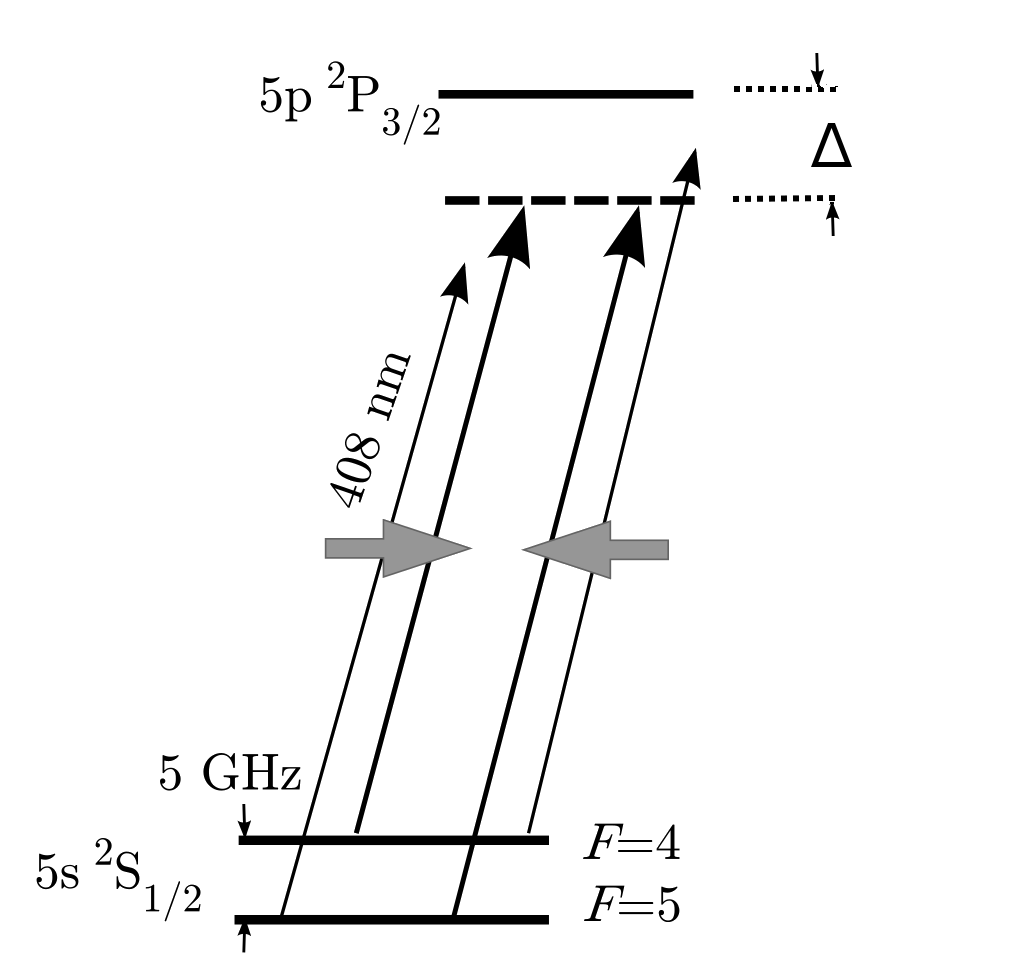
\includegraphics[totalheight=0.3\textheight]{E_level_from_proposal}
}
\caption[Energy level diagram for $^{87}$Sr+]{Energy Level Diagram for $^{87}$Sr+. The hyperfine ground states are separated by a small energy. Diagram is not to scale: a scaled diagram would show the splitting between the $F=4$ and $F=5$ states to be about 147,000 times smaller than the splitting between the $^2$S$_{1/2}$ states and the $^2$P$_{3/2}$ states.}
\label{energyLevelDiagramFigure}
\end{figure}
We now move to a discussion of the dynamics of a three state system, as shown in Figure\,\ref{energyLevelDiagramFigure}. Following Ref.\,\cite{Young1997363}, we write our Hamiltonian as
\begin{equation}
H_{\mathrm{tot}}=H+V.
\end{equation}
Here, $H$ is the Hamiltonian of the atom without the influence of the radiation from the laser. The symbol $V$ represents the interaction between the atom and the laser. 

For present purposes, we neglect all but three states of $H$ ($|e\rangle$,$|g_0\rangle$,and $|i\rangle$). We write $H$ as 
\begin{equation}
H=
\hbar\omega_e |e\rangle\langle e | +
\hbar\omega_g |g\rangle\langle g | +
\hbar\omega_i |i\rangle\langle i | 
\end{equation}
Here, $|e\rangle$,$|g\rangle$, and $|i\rangle$ represent particular internal states of the atom. The state $|i\rangle$ is the ``intermediate state'' and is higher in energy than $|e\rangle$ or $|g\rangle$, which are the two states where we hope and expect to have population buildup. They are all eigenstates of $H$. In Section\,\ref{figureOutStatesSection} we will show that $|e\rangle$ can represent the $F=4$, $m_f=0$, $^2$S$_{1/2}$ state, $|g\rangle$ can represent the $F=5$, $m_f=0$, $^2$S$_{1/2}$ state, and $|i\rangle$ can represent the $F=5$, $m_f=1$, $^2$P$_{3/2}$ state.\footnote{Our analysis applies equally well to other sets of three states within the ions. We can select which states are involved by adjusting the tuning and polarization of the lasers.} See Figure\,\ref{energyLevelDiagramFigure}. The energies of these states are represented by $\hbar\omega_e$, $\hbar\omega_g$, and $\hbar\omega_i$ respectively. 

The term representing the interaction between the laser and the ions is given by
\begin{equation}
V=-\mathbf{d}\cdot\mathbf{E}.
\end{equation}
We model the laser as a classical, oscillating electric field, $\mathbf{E}$, while $\mathbf{d}$ represents the dipole moment matrix operator of our atomic system. The electric field at the location of our atom takes the form 
\begin{equation}
\mathbf{E}=\frac{1}{2}\left(\mathbf{E_1} e^{i\omega_1 t} + \mathbf{E_2} e^{i\omega_2 t} + c.c. \right). \label{eqn:Efield}
\end{equation}
%\mathbf{E_2} \cos(\omega_2t + \phi_2). \label{eqn:Efield}
%oh, it's different phases for the different components of $\mathbf{E_1}.
Here, $\mathbf{E_1}$ and $\mathbf{E_2}$ are complex vectors containing the electric field magnitude, polarization, and relative phase information for two different lasers that oscillate with angular frequencies $\omega_1$ and $\omega_2$ respectively. The symbol $c.c.$ should be taken to mean the complex conjugate of all the terms that came before. We choose to let $\omega_1>\omega_2$. 
Thus, in our convention, the laser with electric field $\mathbf{E_1}$ that oscillates at frequency $\omega_1$ is tuned closer to the transition between $|g\rangle$ and $|i\rangle$, while the $\mathbf{E_2}$, $\omega_2$ laser is tuned closer to the transitions involving $|e\rangle$ and $|i\rangle$. Conveniently, this numbering matches both the conventions in Ref.\,\cite{Young1997363} and it matches the numbering scheme of the slave lasers that is used in Chapter\,\ref{LaserSystemOverview} (i.e. slave 1 outputs a higher frequency than slave 2). 

The dipole moment matrix operator represents the coupling between the laser and the atomic system. The physical details of the dipole moment matrix operator as it relates to the $^{87}Sr^+$ ions will be addressed in Section\,\ref{ElectricDipoleInteraction}. 
However, for now, we make a few physically valid assumptions to simplify our analysis. First, we note that by writing the interaction between the lasers and the atoms in the form $\mathbf{d}\cdot\mathbf{E}$, we have already assumed that the electric field produced by both lasers is uniform in the regime of the atoms. This is known as the ``electric dipole approximation.'' Second, we now assume that all of the on-diagonal dipole moment matrix elements are zero \cite{cohenTannoudji}. Finally, we neglect any possible coupling between $|e\rangle$ and $|g\rangle$. That is to say that $\langle e|\mathbf{d}\cdot\mathbf{E}|g\rangle=0$, or that $V$ only couples $|e\rangle$ and $|g\rangle$ to the intermediate state $|i\rangle$. This assumption is justified by the fact that, first of all, in our particular ions, it works out that $|e\rangle$ and $|g\rangle$ are not dipole-allowed transitions. However, we also note that the laser will be at such a frequency that even states that are dipole allowed will not have any light close enough to their resonances to make them want to transition. Therefore, we expect to be able to write the dipole matrix element operator as 
\begin{equation}
\label{VSchrod}
V=
%\begin{blockarray}{cccc}
%&|e\rangle & |g\rangle & |i\rangle\\
%&\langle e| & \langle g| & \langle i|\\
%\begin{block}{c[ccc]}
\begin{bmatrix}
%|e\rangle & 
0 & 0 & \langle e |\mathbf{d}\cdot\mathbf{E}|i\rangle\\
%|g\rangle & 
0 & 0 & \langle g |\mathbf{d}\cdot\mathbf{E}|i\rangle\\
%|i\rangle & 
\langle i |\mathbf{d}\cdot\mathbf{E}|e\rangle & \langle i |\mathbf{d}\cdot\mathbf{E}|g\rangle& 0 \\
\end{bmatrix}.
%\end{block} 
%\end{blockarray}.
\end{equation}
Here, we have used the basis $|e\rangle$ ,$|g\rangle$, $|i\rangle$. 
%The columns and rows are labeled accordingly.
It is convenient to define the one photon, on-resonance Rabi frequencies:
\begin{align}
\label{RabiFrequencies1}
\Omega_e&=-\frac{\langle i | \mathbf{d}\cdot \mathbf{E}_2 | e\rangle }{\hbar}\\
\Omega_g&=-\frac{\langle i | \mathbf{d}\cdot \mathbf{E}_1 | g\rangle}{\hbar}.
\label{RabiFrequencies2}
\end{align}
%These are called the one photon on-resonance Rabi frequencies.
Now $V$ can be written slightly more concisely as 
\begin{equation}
\label{VSchrod2}
V=-\hbar
%\begin{blockarray}{cccc}
%&|e\rangle & |g\rangle & |i\rangle\\
%&\langle e| & \langle g| & \langle i|\\
%\begin{block}{c[ccc]}
\begin{bmatrix}
%|e\rangle & 
0 & 0 & \Omega_e^*\\
%|g\rangle & 
0 & 0 & \Omega_g^*\\
%|i\rangle & 
\Omega_e & \Omega_g & 0 \\
\end{bmatrix}.
%\end{block} 
%\end{blockarray}.
\end{equation}

%I should have been using \eqref all along 
\subsubsection{Transformation to interaction picture}
First, we move to the interaction picture.
Information on the interaction picture and the basics of quantum dynamics can be found in Refs.\,\cite{sakurai} and \cite{merzbacher}. Moving to the interaction picture is analogous to moving to a so-called ``rotating frame'' as is done in Ref.\,\cite{Young1997363}.The interaction picture is related to the Schr\"odinger picture by the following transformations: 
\begin{align}
\label{intTransforms}
|e\rangle_I&=e^{iH_0t/\hbar}|e\rangle\\
|g\rangle_I&=e^{iH_0t/\hbar}|g\rangle\\
|i\rangle_I&=e^{iH_0t/\hbar}|i\rangle\\
V_I&=e^{iH_0t/\hbar}Ve^{-iH_0t/\hbar}.
\end{align}
In general, we may let $|\psi\rangle$ represent any generic state in the Schr\"odinger picture and $|\psi\rangle_I=\exp(iH_0t/\hbar)|e\rangle$ represent the interaction picture version of the state. The equations of motion satisfied by the states is 
\begin{equation}
i\hbar \frac{\partial}{\partial t}|\psi\rangle_I= V_I|\psi\rangle_I.
\end{equation}
 Note that in the basis $|e\rangle$,$|g\rangle$,$|i\rangle$, we can write $\exp(iH_0t/\hbar)$ as 
\begin{equation}
\label{expH0}
\exp(iH_0t/\hbar)=e^{i\omega_e t}|e\rangle\langle e|+e^{i\omega_g t}|g\rangle \langle g|+e^{i\omega_i t}|i\rangle\langle i|.
\end{equation}
This has the effect of moving the trivial evolution of the ion into the operators and allowing the stationary states of $H$ to have no time-dependent phase. Now, the state of the system may be written as  
\begin{equation}
|\psi(t)\rangle_I = c_e(t)|e\rangle_I+c_g(t)|g\rangle_I+c_i(t)|i\rangle_I,
\end{equation}
where $c_e,c_g,c_i$ are coefficients that change relatively slowly compared to the laser frequencies $\omega_1$ and $\omega_2$.

\begin{table}[h!]
\centering
\begin{tabular}{|c|l|}
\hline
Frequencies & Definition and comment \\ \hline \hline
$\omega_1,\omega_2$& Laser frequencies\\ \hline
$\delta$ & Two photon detuning, $\delta=(\omega_e-\omega_g)-(\omega_1-\omega_2)$\\ \hline
$\Delta,\Delta_{1g},\Delta_{2e}$& One photon detunings, $\Delta\approx\Delta_{1g}=\omega_i-\omega_g-\omega_1\approx
\Delta_{2e}=\omega_i-\omega_e-\omega_2$\\ \hline
$\Omega_{e},\Omega_{g}$ & On-resonance single-photon Rabi frequencies. \\ \hline
$\Omega_{r}$ & Off-resonance Rabi frequency for two photon transition.\\ \hline
$\Omega_{\mathit{eff}}$ & Effective Rabi frequency for two photon transition.\\ \hline
\end{tabular}
\caption{Frequencies used in this derivation. Note that $\omega_1,\omega_2\gg \delta \gg \Delta$. }
\label{frequencyTable}
\end{table}

\subsubsection{Rotating wave approximation}

In order to solve for the dynamics, we must apply the rotating wave approximation. 
%todo: cite Rabi? Sure. 
In order to do this, we first rewrite $\mathbf{E}$ from Eq.\,\ref{eqn:Efield} as 
\begin{multline}
\label{Ebreakdown}
\mathbf{E}=\mathbf{E_1}\frac{\exp(i (\omega_1 t + \phi_1))+\exp(-i(\omega_1 t +\phi_1))}{2}\\
+\mathbf{E_2}\frac{\exp(i (\omega_2 t + \phi_2))+\exp(-i(\omega_2 t +\phi_2))}{2},
\end{multline}
which means that the first few terms of $V_I$ can be written in the interaction picture as
%The thing to copy and paste. 
%\frac{1}{2}e^{i(\omega_x-\omega_y+\omega_z)t+\phi_z}\langle x|\mathbf{d}\cdot\mathbf{E}_z| y\rangle + \frac{1}{2}e^{i(\omega_x-\omega_y-\omega_z)t-\phi_z}\langle x|\mathbf{d}\cdot\mathbf{E}_z| y\rangle
\begin{multline}
\label{Vbreakdown}
V_I=\frac{1}{2}e^{i(\omega_e-\omega_i+\omega_1)t+\phi_1}|e\rangle\langle e|\mathbf{d}\cdot\mathbf{E}_1| i\rangle\langle i | + \frac{1}{2}e^{i(\omega_e-\omega_i-\omega_1)t-\phi_1}|e\rangle\langle e|\mathbf{d}\cdot\mathbf{E}_1| i\rangle\langle i| \\
+
\frac{1}{2}e^{i(\omega_e-\omega_i+\omega_2)t+\phi_2}|e\rangle\langle e|\mathbf{d}\cdot\mathbf{E}_2| i\rangle\langle i| + \frac{1}{2}e^{i(\omega_e-\omega_i-\omega_2)t-\phi_2}|e\rangle\langle e|\mathbf{d}\cdot\mathbf{E}_2| i\rangle\langle i| +
\ldots
\end{multline}
The rotating wave approximation is to assume that only the slowly-oscillating terms will make non-zero contributions to the dynamics of the system. %\cite{Young1997363}. %maybe Griffiths?
The only terms where this criterion is satisfied are the ones near our resonances. 
We have assumed that $\omega_i-\omega_g\approx\omega_1$ and that $\omega_i-\omega_e\approx\omega_2$, which means that our new $V_I$ with the rotating wave approximation applied is
\begin{multline}
V_I=\frac{1}{2}e^{i(\omega_i-\omega_g-\omega_1)t+\phi_1}|i\rangle\langle i|\mathbf{d}\cdot\mathbf{E}_1| g\rangle\langle g | + \frac{1}{2}e^{i(\omega_g-\omega_i+\omega_1)t-\phi_1}|g\rangle\langle g|\mathbf{d}\cdot\mathbf{E}_1| i\rangle\langle i| \\
+
\frac{1}{2}e^{i(\omega_i-\omega_e-\omega_2)t+\phi_2}|i\rangle\langle i|\mathbf{d}\cdot\mathbf{E}_2| e\rangle\langle e| + \frac{1}{2}e^{i(\omega_e-\omega_i+\omega_2)t-\phi_2}|e\rangle\langle e|\mathbf{d}\cdot\mathbf{E}_2| i\rangle\langle i| 
\end{multline}

For convenience, we define the following frequencies: 
\begin{align}
\label{frequencyDiffs}
\Delta_{1g}&=\omega_i-\omega_g-\omega_1\\
\Delta_{2e}&=\omega_i-\omega_e-\omega_2\\
\delta&=(\omega_e-\omega_g)-(\omega_1-\omega_2).
\end{align}
(Table\,\ref{frequencyTable} summarizes most of the relevant frequencies we have defined.) We assume that $\delta\ll\Delta_{1g}$ and that $\delta\ll\Delta_{2e}$, and that $\Delta_{1g}\approx\Delta_{2e}$.

We can write $V_I$ explicitly using Eqs.\,\eqref{Vbreakdown}, \eqref{frequencyDiffs}, \eqref{VSchrod2}, \eqref{RabiFrequencies1}, and \eqref{RabiFrequencies2}:
\begin{equation}
\label{VI_matrix_simplified}
V_I=
\hbar
\begin{bmatrix}
0 & 0 & -\frac{\Omega_e^*}{2}e^{-i\Delta_{2e}t} \\
0 & 0 & -\frac{\Omega_g^*}{2}e^{-i\Delta_{1g}t}\\
-\frac{\Omega_e}{2}e^{i\Delta_{2e}t} & -\frac{\Omega_{g}}{2}e^{i\Delta_{1g}t} & 0 \\
\end{bmatrix}.
\end{equation}

\subsubsection{Adiabatic elimination of $|i\rangle$ state}
In order to solve the system, we use adiabatic elimination to make this look like the two state system. There are several ways to do this. One method is to write the solution as 
\begin{equation} 
|\psi\rangle = 
\begin{bmatrix}c_e(t)\\c_g(t)\\c_i(t)
\end{bmatrix},
\end{equation}
then find the three coupled differential equations that describe the evolution of the system and solve them assuming that $\frac{\partial c_i(t)}{\partial t}=0$. There are some subtleties to this method\footnote{For example, if we had defined our coefficients in terms of the basis vectors of the interaction picture (i.e. so that 
$|\psi\rangle_I=c_{e,I}(t)e^{-iHt/\hbar}|e\rangle+c_{g,I}(t)e^{-iHt/\hbar}|g\rangle+c_{i,I}(t)e^{-iHt/\hbar}|i\rangle$), assuming that $\dot{c}_{i,I}=0$ would not give the right answer.} that are well-explained in Ref.\,\cite{brionLambdaAdiabatic}. In fact, Ref.\,\cite{brionLambdaAdiabatic} gives an excellent discussion of adiabatic elimination for a three state system like ours. 
%Ref.\,\cite{brionLambdaAdiabatic} also describes a method using Green's functions as explained in \cite{cohenTannoudji}. This method involves using the resolvent and projection operators to describe the system. The Green's function of the system is defined as 
%\begin{equation}
%G(z)=\frac{1}{z-\mathbf{H}},
%\end{equation}
%where $z$ is a parameter over which we will eventually integrate and $H$ represents the Hamiltonian of the system. This is to be interpreted essentially as 
%\begin{equation}
%\frac{1}{z-H}=\left(z\mathds{1}-\mathbf{H}\right)^{-1}.
%\end{equation}
%The time evolution of the system can be written as a contour integral in the complex plane:
%\begin{equation}
%U(t)=\frac{1}{2\pi i}\int_{C_+\cup C_-}dz e^{-izt/\hbar}G(z),
%\end{equation}
%where $U(t)$ is the time evolution operator and $C_+\cup C_-$ is a contour integral taken from $-\infty$ to $\infty$ where $C_-$ is just below the real axis that points in the positive real direction and $C_+$ is a contour just above the real axis that points towards the negative real numbers. 
%If we define two projections operators, $P=|e\rangle\langle e| + |g\rangle\langle g|$ and $Q=|i\rangle\langle i|$, it is shown in Ref.\,\cite{cohenTannoudji} that $G(z)$ can be written as 
%\begin{equation}
%PG(z)P=\frac{P}{z-PH_0P-P\left(V+V\frac{Q}{z-QH_0Q-QVQ}V\right)P}.
%\end{equation}
%Ref.\,\cite{brionLambdaAdiabatic} then shows that poles of a certain order can be omitted in the ``pole approximation.'' 

We can also motivate our use of the two state equations of motion using time-dependent perturbation theory. If we take the standard, time-dependent perturbation to second order, we get
\begin{equation}
U_I(t)=\mathds{1}-\frac{i}{\hbar}\int_{t_0}^t dt' V_I(t') + \left(-\frac{i}{\hbar}\right)^2 \int_{t_0}^t dt' V_I(t')\int_{t_0}^{t'}dt'' V_I(t'').
\label{2ndOrderPerturbation}
\end{equation}
The symbol $U_I(t)$ represents the time evolution operator.
If we use Eq.\,\eqref{VI_matrix_simplified} to write $V_I$ in its matrix form, Eq.\,\eqref{2ndOrderPerturbation} becomes
\begin{multline}
U_I(t)=\mathds{1}+i\int_{t_0}^t dt'
\begin{bmatrix}
0 & 0 & \frac{\Omega_e^*}{2}e^{-i\Delta_{2e}t} \\
0 & 0 & \frac{\Omega_g^*}{2}e^{-i\Delta_{1g}t}\\
\frac{\Omega_e}{2}e^{i\Delta_{2e}t} & \frac{\Omega_{g}}{2}e^{i\Delta_{1g}t} & 0 \\
\end{bmatrix}
+ \\
\int_{t_0}^t dt' 
\int_{t_0}^{t'}dt'' 
\begin{bmatrix}
0 & 0 & \frac{\Omega_e^*}{2}e^{-i\Delta_{2e}t'} \\
0 & 0 & \frac{\Omega_g^*}{2}e^{-i\Delta_{1g}t'}\\
\frac{\Omega_e}{2}e^{i\Delta_{2e}t'} & \frac{\Omega_{g}}{2}e^{i\Delta_{1g}t'} & 0 \\
\end{bmatrix}
\begin{bmatrix}
0 & 0 & \frac{\Omega_e^*}{2}e^{-i\Delta_{2e}t''} \\
0 & 0 & \frac{\Omega_g^*}{2}e^{-i\Delta_{1g}t''}\\
\frac{\Omega_e}{2}e^{i\Delta_{2e}t''} & \frac{\Omega_{g}}{2}e^{i\Delta_{1g}t''} & 0 \\
\end{bmatrix},
\end{multline}
which reduces to 

\begin{multline}
U_I(t)=\mathds{1}+i\int_{t_0}^t dt'
\begin{bmatrix}
0 & 0 & \frac{\Omega_e^*}{2}e^{-i\Delta_{2e}t'} \\
0 & 0 & \frac{\Omega_g^*}{2}e^{-i\Delta_{1g}t'}\\
\frac{\Omega_e}{2}e^{i\Delta_{2e}t'} & \frac{\Omega_{g}}{2}e^{i\Delta_{1g}t'} & 0 \\
\end{bmatrix}
+ \\
\int_{t_0}^t dt' 
\int_{t_0}^{t'}dt'' 
\begin{bmatrix}
\frac{|\Omega_e|^2}{4}e^{i\Delta_{2e}(t''-t')} & \frac{\Omega_g\Omega_e^*}{4}e^{i(\Delta_{1g}t''-\Delta_{2e}t')} & 0 \\
\frac{\Omega_g^*\Omega_e}{4}e^{i(\Delta_{2e}t''-\Delta_{1g}t')} & \frac{|\Omega_g|^2}{4} e^{i\Delta_{1g}(t''-t')}& 0\\
0 & 0 & \frac{|\Omega_e|^2}{4}e^{i\Delta_{2e}(t'-t'')}+\frac{|\Omega_g|^2}{4}e^{i\Delta_{1g}(t'-t'')}\\
\end{bmatrix}.
\end{multline}
After carrying out the integration in the variable $t''$, we end up with the following:
\begin{multline}
U_I(t)=\mathds{1}+i\int_{t_0}^t dt'
\left[\begin{smallmatrix}
0 & 0 & \frac{\Omega_e^*}{2}e^{-i\Delta_{2e}t} \\
0 & 0 & \frac{\Omega_g^*}{2}e^{-i\Delta_{1g}t}\\
\frac{\Omega_e}{2}e^{i\Delta_{2e}t} & \frac{\Omega_{g}}{2}e^{i\Delta_{1g}t} & 0 \\
\end{smallmatrix}\right]
+ \\
\int_{t_0}^t dt' 
\left[
\begin{smallmatrix}
\frac{|\Omega_e|^2}{4i\Delta_{2e}}\left(\cancelto{1}{e^{i\Delta_{2e}(t'-t')}}-e^{i\Delta_{2e}(t_0-t')}\right)
 & \frac{\Omega_g\Omega_e^*}{4i\Delta_{1g}}\left(e^{i(\Delta_{1g}-\Delta_{2e})t'}-e^{i(\Delta_{1g}t_0-\Delta_{2e}t')}\right) & 0 \\
\frac{\Omega_g^*\Omega_e}{4i\Delta_{2e}}\left(e^{i(\Delta_{2e}-\Delta_{1g})t'}-e^{i(\Delta_{2e}t_0-\Delta_{1g}t')}\right) 
& \frac{|\Omega_g|^2}{4i\Delta_{1g}}\left(\cancelto{1}{e^{i\Delta_{1g}(t'-t')}}-e^{i\Delta_{1g}(t_0-t')}\right)
& 0\\
0 & 0 & \begin{smallmatrix}
\frac{|\Omega_e|^2}{4i\Delta_{2e}}\left(\cancelto{1}{e^{i\Delta_{2e}(t'-t')}}-e^{i\Delta_{2e}(t'-t_0)}\right) + 
\\ \frac{|\Omega_g|^2}{4i\Delta_{1g}}\left(\cancelto{1}{e^{i\Delta_{1g}(t'-t')}}-e^{i\Delta_{1g}(t'-t_0)}\right)\end{smallmatrix}\\
\end{smallmatrix}
\right].\label{blastedIntegral}
\end{multline}
We now argue that the many terms in this integral that oscillate with frequencies near $\Delta_{2e}\approx\Delta_{1g}$ can be neglected. Instead, we assume that the main contributions will be from the terms that oscillate with frequencies of $0$ or $\Delta_{1g}-\Delta_{2e}$ (which is much smaller than $\Delta_{2e}$ and $\Delta_{1g}$). The reasoning is that the terms that oscillate near $\Delta$ will oscillate through many periods over timescales over which the other terms will be more or less constant. Therefore, we can expect that for the purposes of integrating, the high frequency contributions will be approximately 0.

After removing the terms we are neglecting from Eq.\,\eqref{blastedIntegral} and making the substitutions $\Delta_{2e}-\Delta_{1g}\rightarrow\delta$, $\Delta_{2e}\rightarrow\Delta$, $\Delta_{1g}\rightarrow\Delta$ (we note that $\delta$ is small), we end up with 
\begin{equation}
U_I(t)=\mathds{1} -i \int_{t_0}^{t} dt'
\begin{bmatrix}
\frac{|\Omega_e|^2}{4\Delta} & \frac{\Omega_g\Omega_e^*}{4\Delta}e^{-i\delta t'} & 0 \\
\frac{\Omega_g^*\Omega_e}{4\Delta}e^{i\delta t'} & \frac{|\Omega_g|^2}{4\Delta} & 0 \\
0 & 0 & \frac{|\Omega_e|^2}{4\Delta} + \frac{|\Omega_g|^2}{4\Delta} \\
\end{bmatrix}
\end{equation}
Now, we notice that this very closely resembles the \emph{first}-order Dyson series we would have gotten if we had had a different $V_I$, namely 
\begin{equation}
V_I=
\hbar\begin{bmatrix}\frac{|\Omega_e|^2}{4\Delta} & \frac{\Omega_g\Omega_e^*}{4\Delta}e^{-i\delta t'} & 0 \\
\frac{\Omega_g^*\Omega_e}{4\Delta}e^{i\delta t'} & \frac{|\Omega_g|^2}{4\Delta} & 0 \\
0 & 0 & \frac{|\Omega_e|^2}{4\Delta} + \frac{|\Omega_g|^2}{4\Delta} \\
\end{bmatrix}.\label{newVI0}
\end{equation}
We notice that in the limit we have selected, our new $V_I$ no longer has any terms that might couple a long-term population to the intermediate state $|i\rangle$. Therefore, we will adopt a truncated version of Eq.\,\eqref{newVI0} as our interaction Hamiltonian. What I have presented is not an airtight argument, but the result is correct. Alternative justifications for this can be found in several places, most helpfully in Ref.\,\cite{brionLambdaAdiabatic}.

We will now treat this like a two-state system, so from now on we let 
\begin{equation}
V_I=
\hbar
%\begin{blockarray}{ccc}
%&|e\rangle & |g\rangle & |i\rangle\\
%&\langle e| & \langle g|\\
%\begin{block}{c[cc]}
\begin{bmatrix}
%|e\rangle & 
\frac{|\Omega_e|^2}{4\Delta} & \frac{\Omega_g\Omega_e^*}{4\Delta}e^{-i\delta t'}\\
%|g\rangle &
 \frac{\Omega_g^*\Omega_e}{4\Delta}e^{i\delta t'} & \frac{|\Omega_g|^2}{4\Delta}\\
\end{bmatrix},\label{newVI}
%\end{block}
%\end{blockarray}.
\end{equation}
where we have written our matrix in the $|e\rangle$, $|g\rangle$ basis.\footnote{Notice that we are not writing $V_I$ in the $|e\rangle_I$, $|g\rangle_I$ basis. These are the $|e\rangle$ and $|g\rangle$ states that are not time-dependent. The time-dependence of $V_I$ is explicit in the matrix coefficients.}
Now, the solution to this equation is very similar to the solution to the two state system discussed in \ref{twoStateSection}. Here, the quantity analogous to the off-resonance Rabi frequency is given by \cite{Young1997363}: 
\begin{equation}
\Omega_\mathit{r}=\sqrt{\Omega_\mathit{eff}^2+(\delta-\delta^{AC})^2},
\end{equation}
where $\delta^{AC}= \frac{|\Omega_e|^2}{4\Delta}-\frac{|\Omega_g|^2}{4\Delta}$. This frequency accounts for the AC Stark shifts that appeared in Eq.\eqref{newVI}. Also, $\Omega_{\mathit{eff}}$ is the effective on-resonance Rabi frequency given by 
\begin{equation}
\Omega_{\mathit{eff}}=\frac{\Omega_e^*\Omega_g}{2\Delta}.
\end{equation}
%do I need a phase in here? 
%(\Omega_e^{AC}-\Omega_g^{AC})$. The symbols $\Omega_e^{AC}$ and $\Omega_g^{AC}$ represent the AC Stark shifts 

Following the analysis of a two-state system, it can be shown that the population in our two states for the case where $|c_g(\tau=0)|^2=1$ and $|c_e(\tau=0)|^2=0$ is given by 
\begin{align}
|c_e(\tau)|^2&
=\frac{\Omega_{\mathit{eff}}^2}{2\Omega_r^2}(1-\cos(\Omega_r\tau))\\
|c_g(\tau)|^2&=
1-\frac{\Omega_{\mathit{eff}}^2}{2\Omega_r^2} + \left(\frac{\Omega_{\mathit{eff}}^2}{2\Omega_r^2}\right)\cos(\Omega_r \tau).
\end{align}
Here again we see that in order to coherently move the entire population, we need to ensure that $\Omega_{\mathit{eff}}=\Omega_r$. This can be accomplished only when $\delta-\delta_{AC}=0$. Notice that the detuning from the upper state $\Delta$ only affects the Rabi rate. As long as it is small enough that our approximations hold, it does not affect the total population transfer that can be achieved. However, if the off-resonance Rabi frequency gets small enough, it is possible that we will run into the practical difficulty of not having enough laser power over a large enough interaction area to effectively transfer the ion population to the desired states.

%Ref.\,\cite{Young1997363} then shows that the effective Rabi frequency, $\Omega_{\mathit{eff}}$ is given by 
%\begin{equation}
%\Omega_{\rm eff}=\frac{\Omega_{e} \Omega_{g}}{2 \Delta},
%\end{equation}
%where $\Delta$ is the one photon detuning. 
%\begin{equation}
%\Omega_\mathit{eff}=\sqrt{\left(\frac{\Gamma^2S_0}{2}\right)^2 + \delta^2}
%\end{equation}

%\begin{equation}
%\Omega = \frac{-eE_0}{\hbar}\langle e |\vec{r}|g\rangle=\frac{\vec{d}E_0}{\hbar}
%\end{equation}

%This is all valid in the case where 
%
%\begin{equation}
%\delta\ll\Delta
%\end{equation}


%In Ref.\ \cite{cjeDiss}, this calculation is performed, but some of the details are left mysterious. In particular, no source is cited for any of the physical parameters of the $^{87}$Sr+ atom (e.g. the dipole moment values, the transition width, the saturation parameter). We hope to reproduce this calculation with more details.  

%\section{States and quantum numbers}
\section{Real world $^{87}$Sr$^+$ Hamiltonian contributions and relevant states}

In this section, we will discuss the states of the real-world Strontium ions that will be used in the experiment. We will discuss the contributions to the Hamiltonian and figure out which states are relevant to the experiment. 

The Hamiltonian of the Strontium ions is analogous to the Hamiltonian of a single-electron atom. 
In a single electron atom, the solution to the Schr\"odinger equation describing the electron is solved by separation of variables.
 Each solution is a product of a spherically symmetric function that depends only on the distance $r$ from the nucleus and the spherical harmonics.
This is because the orbital angular momentum operator $\mathbf{L}$ commutes with such a Hamiltonian. In fact, the orbital angular momentum operator commutes with any Hamiltonian with a spherically symmetric potential.
Thus, we can use the familiar angular momentum quantum numbers for the eigenstates of any spherically symmetrical Hamiltonian.
%keep this?

In the case of $^{87}$Sr+, there is only one electron in the valence band. The inner shells are full and we assume that the symmetry is such that the eigenstates of the atom will also be eigenstates of the orbital angular momentum operator, $\mathbf{L}$.
 The system also involves two other angular momentum operators: the spin operator for the valence electron, $\mathbf{S}$, %\footnote{The spin of the electrons on the inner shells cancels and adds to 0} 
 and the spin of the nucleus, $\mathbf{I}$. 
(Here and throughout, we will use the boldface $\mathbf{I}$ to mean the operator while the unbolded letter ($I$) will mean the associated eigenvalue.)
%We will first approximate the Hamiltonian by assuming that there is no coupling that is dependent on the spin. 
%The hyperfine interaction will be modeled as a perturbation on top of this.

The ``good'' quantum numbers for describing the internal states of a $^{87}$Sr+ ion are $F$, $J$, $L$, $S$, $m_f$ and $n$\cite{experimental_hyperfine_alkali_arimondo}\cite{cuaMITnotes} where $F$, $J$, $L$, $S$, $m_f$ take on their usual meanings (see Table\, \ref{quantumNumberQuickref}). This is because the Hamiltonian for the unperturbed atom is diagonal in this basis. Equivalently,  it is because these operators all commute with one another and with the other pieces of the Hamiltonian. However,  a few of the external stimuli to the ions (like the constant magnetic field or the interaction of the lasers) can be most naturally modelled in terms of the eigenstates of the $L, m_l, S, m_s, I, m_I$ quantum numbers.   

\begin{table}[h!]
\centering
\begin{tabular}{|c|l|}
\hline
Quantum Number & Definition and comment \\ \hline \hline
L & Orbital angular momentum of valence electron. \\ \hline
S & Spin of valence electron. Takes on values $\pm 1/2$ \\ \hline
I & Nuclear spin. For $^{87}$Sr$^+$, $I=9/2$ \\ \hline
J & Total valence electron angular momentum. $\mathbf{J}=\mathbf{L}+\mathbf{S}$ \\ \hline
F & Total angular momentum $\mathbf{F}=\mathbf{I}+\mathbf{J}$ \\ \hline
$m_f$ & Eigenvalue of $\mathbf{F}_z$.\\ \hline
\end{tabular}
\caption{The quantum numbers used to describe the internal state of the $^{87}$Sr+ ion.}
\label{quantumNumberQuickref}
\end{table}

There are two basic things we have to do in this section. First, we must account for each of the contributions to the Hamiltonian of the ions. We will write the Hamiltonian as 
\begin{equation}
H=H_0+H_{\mathrm{hfs}}+H_{\mathrm{Z}},\label{Hoverall}
\end{equation}
where $H$ represents the Hamiltonian of the ion while it is \emph{unperturbed} by the laser. The contribution to the Hamiltonian due to the hyperfine splitting is encapsulated in $H_{\mathrm{hfs}}$, while $H_{\mathrm{Z}}$ represents the contribution that Zeeman shifts make to the Hamiltonian. (We create a constant, but adjustable magnetic field through which the atoms travel during the experiment. We do this specifically to break degeneracies between certain of the levels in the atom as discussed in Section\,\ref{zeeman}.) The rest of the Hamiltonian is represented by $H_0$. We do not explicitly consider other contributions to the Hamiltonian (for example, the fine structure) because these are built into the values we look up in the NIST atomic spectra database \cite{NISTasd}.\footnote{For example, the NIST database gives transition lifetimes for $^2$S$_{1/2}\rightarrow^2$P$_{3/2}$ transitions. The fine structure is already accounted for, as evidenced by the fact that there is a separate entry for $^2$S$_{1/2}\rightarrow^2$P$_{1/2}$ transitions.}

Second, we must find which exact states the experiment will use.
Our experiment is designed to use the $^2$S$_{1/2}$ and $^2$P$_{3/2}$ states. However, each of these spectroscopic terms refers to many states: For example, we must account for the states that correspond to different values of $F$. Since $\mathbf{F}=\mathbf{I}+\mathbf{J}$, $F$ can take on any values between $|I-J|,|I-J|+1,...,|I+J|$. So, for example, since $I=9/2$, the valid values of $F$ for the $^2$S$_{1/2}$ state are $F=4$ and $F=5$. For the upper states, where $J=3/2$, $F$ can take on the values $3,4,5,$ or $6$. We must also take into account the many possible values of $m_J$ and $m_F$ for these states.

\subsection{Review of hyperfine splitting}

We now discuss the Hyperfine contribution to our overall Hamiltonian. We will need to understand the hyperfine splitting to allow us to model the 5 GHz energy difference between the $F=4$ and $F=5$ $^2$S$_{1/2}$ states. Our discussion will allow us to calculate hyperfine shifts for all the energy levels in our atom based on the hyperfine $A$ and $B$ coefficients, for which we have found experimental and numerical estimates in the literature.

\subsubsection{Hyperfine basics}

The hyperfine splitting arises from interactions between the nucleus and the electrons. The piece of the Hamiltonian representing the Hyperfine interaction is represented by the symbol $H_{\mathrm{hfs}}$ in Eq.\,\eqref{Hoverall}.
The standard expansion of $H_{\mathrm{hfs}}$ in the literature is:  
\begin{equation}
H_{\mathrm{hfs}}=\sum_k \mathbf{T}^{(k)} \cdot \mathbf{M}^{(k)} \label{hfs_hamiltonian_eqn},
\end{equation}
where $\mathbf{T}^{(k)}$ and $\mathbf{M}^{(k)}$ are irreducible spherical tensor operators of rank $k$
\cite{schwartz_hyperfine_expansion}
\cite{experimental_hyperfine_alkali_arimondo}
\cite{chinesePhysics}.
The dot product for spherical tensors of arbitrary rank is defined in the normal way as
\begin{equation}\label{TkMk_hyperfine}
\mathbf{T}^{(k)}\cdot\mathbf{M}^{(k)}=\sum_q (-1)^qT_q^{(k)}M_{-q}^{(k)}.
\end{equation}
%\footnote{todo: cite that review article and the lecture notes you found}
The tensor operator $\mathbf{T}^{(k)}$ represents information about the electron.
$\mathbf{M}^{(k)}$ represents the nucleus\cite{experimental_hyperfine_alkali_arimondo}\cite{schwartz_hyperfine_expansion}
\cite{sobelman_spectra}.
Writing the expansion in this form shows explicitly the geometry of the operator. 

Before discussing what information $\mathbf{T}^{(k)}$ and $\mathbf{M}^{(k)}$ represent exactly,
we pause to point out a few geometrical facts. Even if we had no knowledge of the mechanism by which hyperfine interactions occur, we might still arrive at Eq.\,\ref{hfs_hamiltonian_eqn} simply by geometrical considerations.
Notice that the generator of rotations under which $\mathbf{T}^{(k)}$ is valid is the electron total angular momentum, $\mathbf{J}$, while $\mathbf{M}^{(k)}$ is subject to rotations defined in terms of the nuclear angular momentum operator $\mathbf{I}$. 
The direct product of these two gives us a value that can be validly rotated using the group generated by the combined angular momentum operator $\mathbf{F}$.\cite{Racah2}\cite{sobelman_spectra}. Thus, each term of our expansion has two parts: one that is a valid tensor operator associated with the geometry of the nucleus and one that is a valid tensor operator associated with the geometry of the electron. By combining these two parts using a dot product, we see that each term turns out to be a valid tensor operator for the entire atomic system. This is exactly what we would expect.

The most important contributions to the Hyperfine splitting come from magnetic dipole interactions and electric quadrapole interactions \cite{sobelman_spectra}\cite{schwartz_hyperfine_expansion}\cite{cuaMITnotes}. These correspond to the $k=1$ and $k=2$ terms in Eq.\,\eqref{TkMk_hyperfine} respectively\cite{experimental_hyperfine_alkali_arimondo}.
%\footnote{It is interesting to note that the odd values of $k$ correspond to magnetic interactions while the even values correspond to electric interactions. That is to say that there is no electric dipole interaction between the electrons and the nucleus, but there is a magnetic dipole ($k=1$), while there is an electric quadrapole coupling, but no magnetic quadrapole, etc}
\subsubsection{Magnetic dipole interaction}
First, we discuss the $k=1$ term, or magnetic dipole interaction term from the expansion in Eq.\,\eqref{TkMk_hyperfine}. Classically, we know that the potential energy of a dipole in a magnetic field is proportional to the dot product of the magnetic dipole moment vector with the magnetic field vector ($U=-\mathbf{\mu}\cdot\mathbf{B}$). We also know that the magnetic field at the center of a classical dipole points in the direction of the dipole moment. Therefore, it seems reasonable that the energy due to the interaction of the electron and the nucleus might be somehow proportional to a dot product of two vectors representing their respective angular momenta. Indeed, this turns out to be the case: the magnetic dipole interaction can be written as follows\cite{sobelman_spectra}: 
\begin{equation}\label{IdotJ}
W_f=A\mathbf{I}\cdot\mathbf{J},
\end{equation}
where $W_f$ represents the energy associated with this coupling and $A$ encapsulates a coupling factor between the nuclear and electronic magnetic moments. 
%Note that here we are using the normal, three dimensional dot product (i.e. $\mathbf{I}\cdot\mathbf{J}=I_xJ_x+I_yJ_y+I_zJ_z$). 

The product $\mathbf{I}\cdot\mathbf{J}$ can be expanded by noticing that $\mathbf{F}^2=(\mathbf{I}+\mathbf{J})^2=\mathbf{I}^2+2 \mathbf{I}\cdot\mathbf{J}+\mathbf{J}^2$. This gives \cite{cuaMITnotes}\cite{sobelman_spectra}: 
\begin{equation}\label{Wf_dot_product}
W_f=\frac{1}{2}A(\mathbf{F}^2-\mathbf{J}^2-\mathbf{I}^2).
\end{equation}
We can also see how Eq.\,\ref{IdotJ} represents the $k=1$ term in Eq.\,\eqref{TkMk_hyperfine}. We clearly have one tensor operator from the Nuclear angular momentum space ($\mathbf{I}$) along with one vector from the electron angular momentum space ($\mathbf{J}$). The product we get is a scalar that will be invariant under rotations in the total space.\footnote{A quick note about constants. In the expansion in Eq.\,\eqref{TkMk_hyperfine}, there are different conventions \cite{schwartz_hyperfine_expansion} for deciding which coefficients are pulled into which operators. However, as we will see, the coefficient $A$ as used in Eq.\,\ref{IdotJ} is defined in a standard way and can be looked up in the literature. For this reason, we are specifying $T$ and $M$ only up to a constant. This is fine since the point of showing the expansion is really just to make a comment about the geometry of hyperfine interactions, while the actual calculations only involve the first two terms}

\subsubsection{Electric quadrapole interaction}
In a similar way, the $k=2$ term in Eq.\,\eqref{TkMk_hyperfine} can be shown to correspond to the electric quadrapole interaction. Chapter 6.2 of Ref.\,\cite{sobelman_spectra} gives a good explanation for this. The crux of the argument is that the electric quadrapole interaction,
\begin{equation}
W=\int\frac{\rho(\mathbf{r})\rho'(\mathbf{r}')}{|\mathbf{r}-\mathbf{r}'|}d\mathbf{r}d\mathbf{r'}.
\end{equation}
%Should I change this symbol?
can  be expanded in terms of spherical harmonics: 
\begin{equation}
W=\int d\mathbf{r}d\mathbf{r'}
\rho(\mathbf{r})\rho'(\mathbf{r}')\sum_k \frac{r'^k}{r^{k+1}}[C^k(\theta,\phi)\cdot C^k(\theta',\phi')] \label{quadrupole_expanded}.
\end{equation}

The $k=2$ term in the integral contained in Eq.\,\ref{quadrupole_expanded} takes the form of an inner product between two rank 2 spherical tensors. Thus, we are satisfied that we have found the $k=2$ terms in Eq.\,\eqref{TkMk_hyperfine}.

The inner product between two rank 2 spherical tensors can be evaluated using Eq. 4.169 from Sobelman \cite{sobelman_spectra} (the formula can also be found in Ref.\,\cite{Racah2} and is also referred to in Ref.\,\cite{schwartz_hyperfine_expansion}):
\begin{multline}\label{4169_combine_diff_tensors}
\langle\gamma I J F m_f|(T^{(k)}M^{(k)})|\gamma J I F m_f\rangle \\
=
(-1)^{F+I+J} \sum_{\gamma} \langle\gamma J||T^{(k)}||\gamma J\rangle
\langle\gamma I || M^{(k)} ||\gamma I\rangle
\begin{Bmatrix}
J & I & F \\
I & J & k
\end{Bmatrix},
\end{multline}
where 
$\begin{Bmatrix}
J & I & F \\
I & J & k
\end{Bmatrix}$ represents the Wigner $6j$ symbol. 

Using the properties of the Wigner $6j$ symbols, it can be shown that %\footnote{I will get this from Sobelman. He gives the Racah coefficients in 4.97 - 4.99} 
the equation for the electric quadrapole term in the hyperfine interaction takes the form \cite{cuaMITnotes}\cite{sobelman_spectra} 
%\footnote{OK Dallin--I'm not sure if I should even include this.} 
\begin{equation}\label{justQuadrupole}
W=BC(C+1),
\end{equation}
where 
\begin{equation}
C=F(F+1)-J(J+1)-I(I+1).
\end{equation}
(Interestingly, Eq.\,\ref{Wf_dot_product} can also be evaluated using Eq.\,\ref{4169_combine_diff_tensors} using $k=1$.)

\subsubsection{Write both hyperfine terms in terms of standard constants}
We can rewrite Eq.\,\eqref{Wf_dot_product} in terms of $C$ 
and then combine it with Eq.\,\eqref{justQuadrupole} to get the full hyperfine splitting\cite{cuaMITnotes}: 
\begin{equation}\label{Standard_hyperfine_AB}
E_{\mathrm{hfs}}=\frac{1}{2}AC+BC(C+1).
\end{equation}
The coefficients $A$ and $B$ as used in Eqs.\,\ref{Standard_hyperfine_AB} and \ref{Wf_dot_product} are the hyperfine A and B coefficients.\footnote{These are \emph{not} the Einstein $A$ and $B$ coefficients relating to radiative transition rate. Though, unfortunately, we will have to mention the Einstein $A$ and $B$ coefficients later.} The symbols $A$ and $B$ are a standard name and notation used in calculating hyperfine energy shifts. Their values can be looked up in the literature\cite{cuaMITnotes}.  We found values for the $A$ and $B$ coefficients for $^{87}$Sr+ in Ref.\,\cite{safronova2photon}. These are summarized in Table\,\ref{AB_table}.  

\begin{table}[h]
\centering
\begin{tabular}{|l|r|r|r|}
\hline
Level &  $A^{\mathrm{(SDpT)}}$ &$A^{\mathrm{(theor)}}$ & $A^{\mathrm{(expt)}}$ \\ \hline \hline
$5s ^2$S$_{1/2}$&-997.85 MHz& -1000 MHz& -1000.473673(11) MHz\\ \hline
$5p ^2$P$_{3/2}$&-35.26 MHz&-35.3 MHz&-36.0(04) MHz\\ \hline
\end{tabular}

\begin{tabular}{l}
%\quad \\
\end{tabular}

\begin{tabular}{|l|r|r|r|}
\hline
Level &  $B^{\mathrm{(SDpT)}}$ &$B^{\mathrm{(theor)}}$ & $B^{\mathrm{(expt)}}$ \\ \hline \hline
$5s ^2$S$_{1/2}$&&0  MHz&  \\ \hline
$5p ^2$P$_{3/2}$&88.94MHz&$88.68$MHz\footnotemark&88.5(54)MHz \\ \hline
\end{tabular}
\caption{Values of A and B coefficients in MHz for relevant states taken from Ref.\,\cite{safronova2photon}. The label ``SDpT'' refers to the value calculated using one particular numerical approach as detailed in Ref.\,\cite{safronova2photon}. The label ``theor'' represents theoretically calculated values. The label ``expt'' refers to measured values from experiments.\label{AB_table}
}
\end{table}
\footnotetext{Ref.\cite{safronova2photon} reports $B/Q$ as 271MHz$/$b and also says that $Q=0.327(24)$b. We multiplied 271MHz$/$b$\times 0.327(24)$b$=88.68$ MHz, to get the value that appears here.}%NOTICE: IDK how to get this footnote to be guaranteed to appear on the right page.}

\subsubsection{Calculate hyperfine energy shifts}
We may calculate the splitting between the $F=4$ and $F=5$ $^2$S$_{1/2}$ states using $I=9/2$, $F=4,5$, $L=0$ using Eq.\,\ref{Standard_hyperfine_AB}. In this case, we can see that with $A=1000$MHz, we can calculate the splitting between the $F=4$ and $F=5$ levels: 
\begin{align}
C_{F=4} &= -5.5\\
C_{F=5} &= 4.5\\
W_{F=4}-W_{F=5}&=5000 \quad \mathrm{MHz}.
\end{align}

Furthermore, we can calculate the hyperfine splitting for all the $^2$P$_{3/2}$ states, which is contained in Table \ref{tableOfHyperfinedeetuings}.

\begin{table}[h]
\centering
\begin{tabular}{|l|l|}
\hline
State & Hyperfine shift  \\ \hline \hline
%$F=4$ $^2$S$_{1/2} (5s)$ & Ground state  \\ \hline
%$F=5$ $^2$S$_{1/2} (5s)$ & Ground state  \\ \hline
$F=3$ $^2$P$_{3/2} (5p)$ & 22971  MHz\\ \hline
$F=4$ $^2$P$_{3/2} (5p)$ &  5803 MHz\\ \hline
$F=5$ $^2$P$_{3/2} (5p)$ &  306 MHz\\ \hline
$F=6$ $^2$P$_{3/2} (5p)$ &   17121 MHz\\ \hline
\end{tabular}
\caption{Hyperfine splitting on $^2$P$_{3/2}$ states. The Hyperfine shift represents the energy shift between the Hamiltonian neglecting hyperfine splitting and the Hamiltonian that includes it
%\footnote{Actually, there may be either some other offset or some theorem that says these are centered around the original level? That can't be right}
. The values are given in MHz and the associated energy is $hf$. Code for calculating these values can be found in Appendix\,\ref{sympy6jAppendix}.}
\label{tableOfHyperfinedeetuings}
\end{table}

\subsection{Magnetic field}\label{zeeman}

The next feature of our system Hamiltonian that we need to model involves the constant magnetic field pointing in the $\hat{z}$ direction that exists throughout the entire area where the interferometry will take place. This field has been placed there intentionally to break the degeneracy of some of the $m_f$ sub-levels that we might couple to. It also prevents the atoms from precessing around stray magnetic fields, which would take them out of the lab-centric coordinate system we would like to keep them in.

The energy shift due to the Zeeman interaction is simply \cite{sobelman_spectra}: 
\begin{equation}
W=-\mathbf{\mu}\cdot\mathbf{H},
\end{equation}
where $\mathbf{\mu}$ is the magnetic dipole moment of the atom and $\mathbf{H}$ is the magnetic field strength. The magnetic moment $\mathbf{\mu}$ for an atom without hyperfine structure can be written as \cite{sobelman_spectra}
\begin{equation}
\mu=-\mu_0 g \mathbf{J}.
\end{equation}
Here $\mu_0$ is the Bohr Magneton and $g$ is the gyro-magnetic ratio or $g$ factor which is usually of order unity. 

We note that, in contrast to $H_{\mathrm{hfs}}$, which turned out to be diagonal in the $F, I, J, S, m_f$ basis, the interaction energy due to a magnetic field pointing in the $\hat{z}$ direction is more naturally written in the $I, m_I, L, m_L, S, m_S$ basis. This is because the field breaks the degeneracy of the $m_x$ levels and it would be nice to be able to model the effect using the magnetic moment of the electron spin, electron orbit and nuclear spin separately. 

However, we can make an approximation for the case where the Zeeman splitting is small compared to the hyperfine splitting. 
%The overall 
%\begin{equation}
%\mathbf{\mu}=-\mu_0 g \mathbf{J}
%\end{equation}
Ref.\,\cite{sobelman_spectra} gives us the following equation:
\begin{equation} \label{zeemanSobelman}
\langle{\gamma JIFM|W|\gamma JIFM\rangle = \mu_0 g \frac{F(F+1)+J(J+1)-I(I+1)}{2F(F+1)}m_f H},
\end{equation}
where $\mu_0=e\hbar/(2 m_e)$ and is the Bohr magneton.\footnote{$e \hbar / (2 m_e c)$ in Gaussian units} (Here, $m_e$ is the mass of the electron.)

Eq.\,\ref{zeemanSobelman} shows that the Zeeman splitting is linear as a function of $m_f$. The splitting depends on $g$, the Land\'e $g$ factor of the atom and the magnetic field. We expect the Land\'e $g$ factor to be of order $1$. We could perform a more in-depth analysis of the exact splitting. However, in the experiment, the magnetic field is adjustable and will be tuned in such a way that it just barely removes the degeneracy between the $m_f$ sub-levels. In other words, we will adjust $H$ until the separation between adjacent $m_f$ sub-levels is just a few times greater than the line width of our laser, which is on the order of a few hundred Megahertz. Therefore, for the purposes of our calculations here, we will simply assume that the $m_f$ sub-levels for each of our states are not degenerate and that the energies differ by $\sim$100 MHz.

\subsection{Electric dipole interaction with laser light}
%\section{Finding appropriate values in the literature}
%redundant
\label{ElectricDipoleInteraction}
The next piece of the Hamiltonian that we need to model involves the interaction with the laser. Following the work of Section\,\ref{threeStateSystemExplanation}, we still model the laser radiation as a classical field that makes a time-dependent contribution to the Hamiltonian. We also make the electric dipole approximation and we assume that $V$ can be written in terms of a dipole interaction:  \cite{demilleBudkerKimball}\cite{cuaMITnotes}\cite{gustavsonThesis}\cite{Young1997363}
\begin{equation}
H_{\textnormal{int}}=-\mathbf{d}\cdot\mathbf{E},
\end{equation}
%the equation actually comes from Gustavson thesis.
where $\mathbf{E}$ represents the electric field at the atom, %\footnote{which we also assume is constant over the entire length of the atom--this is actually part of the electric dipole approximation} 
and $\mathbf{d}$ represents the dipole moment operator for our states. 

%The classical definition of the electric dipole moment is $\mathbf{p}=q \mathbf{d}$ where $\mathbf{p}$ is a vector representing the dipole moment, $q$ is the charge, and $\mathbf{d}$ is the displacement vector

%\subsubsection{Evaluation of dipole moment operator}
We must now evaluate the dipole moment operator. Specifically, we need to find
\begin{align}
\langle i|\mathbf{d}&\cdot\mathbf{E}|g\rangle \\
\langle i|\mathbf{d}&\cdot\mathbf{E}|e\rangle
\end{align}
in order to calculate $\Omega_e$, $\Omega_g$ and, ultimately, $\Omega_r$.

Classically, the dipole moment is a vector quantity that encapsulates the charges and the distance between them. The dipole moment operator that we are looking should, in the classical limit, equal the charge of the electron times some vector that roughly represents the displacement between the electron and the nucleus. The dipole moment operator is defined as 
\begin{equation}
\mathbf{d}=-e\mathbf{r},
\end{equation}
where $\mathbf{d}$ is the dipole moment operator, $e$ is the fundamental charge.\footnote{in our convention, $e>0$ and the charge of an electron is $-e$} and $\mathbf{r}$ represents the vector operator describing the electron's position relative to the atom\cite{demilleBudkerKimball}

The electric dipole moment operator commutes with the $\mathbf{S}$ and $\mathbf{I}$ operators. The rotation operators that may be used to generate rotations of the electric dipole moment operator are $\mathbf{L}$, $\mathbf{J}$ and $\mathbf{F}$\cite{DeMille_presentation}. In other words, the electric dipole moment operator is most naturally discussed using the $L$ and $m_l$ basis. 

However,  our Hamiltonian is still specified using the $F, J, I, L, m_f$ basis. Thus,  we must perform a change of basis operation on the electron dipole moment operator. In order to do this,  we could use repeated applications of the Wigner-Eckart theorem.  
However, for now it is more convenient if we make use of an equation similar to Eq.\,\ref{4169_combine_diff_tensors} that is known in some places as the ``spectator theorem''\cite{DeMille_presentation}. % Here, we are interested in finding the matrix elements of the dipole operator in terms of the  basis that we have selected.

The theorem says that, given a system with two angular momenta, $\mathbf{J}_1$ and $\mathbf{J}_2$ and total angular momentum $\mathbf{J}_{12}=\mathbf{J}_1+\mathbf{J}_2$,
\begin{multline}\label{spectatorTheorem}
\langle\gamma' J_1'J_2J_{12}'||T^{(k)}||\gamma J_1 J_2 J_{12}\rangle=
\\(-1)^{J_1'+J_2+J+k}\langle\gamma'J_1'||T^{(k)}||\gamma J_1\rangle
\sqrt{2J_{12}+1}\sqrt{2J_{12}'+1}
\begin{Bmatrix}
J_1' & J_{12}' & J_2 \\
J_{12} & J_1 & k
\end{Bmatrix},
\end{multline}
%where we have used $J_{1(2)}$ is the initial quantum number for $\mathbf{J}_{1(2)}$ and $J_{1(2)}'$
where we have used $J_{1}$,$J_{2}$ and $J_{12}$ to refer to the initial values for their respective operators and $J_{1}'$,$J_{2}'$ and $J_{12}'$ correspond to the final values. The parameters $\gamma$ and $\gamma'$ respectively represent the initial and final values of all other quantum numbers that describe the system.

%We will use this formula twice: once to separate out $I$ and $J$ from $F$ and then once to remove $J$ by splitting out the pieces related to $L$ and $S$.
We will use this formula to separate out $I$ and $J$ from $F$.
%credit deMille for the HW problem?
We eliminate $F$, by making the following replacements in Eq.\,\ref{spectatorTheorem}:
\begin{align}
J_1&\rightarrow J\\
J_2&\rightarrow I\\
J_{12}&\rightarrow F\\
\gamma &\rightarrow  n,L,S.
\end{align}
This gives 
\begin{multline}\label{spectatorTheorem1}
\langle n' L' S J' I F'||T^{(k)}||n L S J I F\rangle=
\\(-1)^{J'+I+J+k}\langle n'L' S J'||T^{(k)}|| n L S J\rangle
\sqrt{2F+1}\sqrt{2F'+1}
\begin{Bmatrix}
J' & F' & I \\
F & J & k
\end{Bmatrix}.
\end{multline}
For convenience, we will refer later to 
\begin{equation}
\frac{\langle n' L' S J' I F'||T^{(k)}||n L S J I F\rangle}{\langle n'L' S J'||T^{(k)}|| n L S J\rangle}=(-1)^{J'+I+J+k}\sqrt{2F+1}\sqrt{2F'+1}
\begin{Bmatrix}
J' & F' & I \\
F & J & k
\end{Bmatrix}.
\label{afterSpectators}
\end{equation} 
Table\,\ref{coefficient_calculated} contains several relevant, calculated values of this quantity.

We could use Eq.\,\ref{spectatorTheorem} again, making additional substitutions in order to get an expression that relates $\langle n' L' S J' I F' ||\mathbf{r}||n L S J I F\rangle$ to $\langle n' L'||\mathbf{r}||n L \rangle$. In some ways, this would be the most natural thing to do since the electric dipole moment is associated with $L$ and is not related to electron spin. As we mentioned before, the electron spin operator $\mathbf{S}$ commutes with the electric dipole operator. In this sense, the electron spin is a so-called ``spectator'' operator that could be accounted for with the spectator theorem (as we have just done with $F$). However, it turns out that values for the reduced electric dipole moment matrix operator that we found in the literature (this is discussed in Section \ref{lookItUp}) are given in the $J$ basis (i.e. $\langle n'L'S J'||d^{(k)}||n L S J I F\rangle$).

%Next, we would make the following substitutions: 
%
%\begin{align}
%J_1&\rightarrow L\\
%J_2&\rightarrow S\\
%J_{12}&\rightarrow J\\
%\gamma & \rightarrow n
%\end{align}
%
%\begin{multline}\label{spectatorTheorem2}
%\langle\gamma L'SJ'||T^{(k)}||\gamma L S J\rangle=
%\\(-1)^{L'+S+L+k}\langle\gamma'L'||T^{(k)}||\gamma L\rangle
%\sqrt{2J+1}\sqrt{2J'+1}
%\begin{Bmatrix}
%L' & J' & S \\
%J & L & k
%\end{Bmatrix}
%\end{multline}
%
%Combining Eqs.\,\ref{spectatorTheorem1} and \ref{spectatorTheorem2} gives 

%\begin{multline} \label{afterSpectators}
%\langle n' L' S J' I F' ||\mathbf{r}||n L S J I F\rangle = \\
%(-1)^{J'+I+J+k+L'+S+L+k}
%\sqrt{2F+1}\sqrt{2F'+1}\sqrt{2J+1}\sqrt{2J'+1} \quad \times \\
%\begin{Bmatrix}
%J' & F' & I\\
%F & J & k
%\end{Bmatrix}
%\begin{Bmatrix}
%L' & J' & S\\
%J & L & k
%\end{Bmatrix}
%\langle \gamma' L' ||\mathbf{r}^{(k)}|| \gamma L\rangle 
%\end{multline}
Now, we can calculate the Wigner 6j symbols using the SymPy module in Python\cite{sympy}\cite{rasch6j}.
 %\footnote{not sure how to cite: \url{http://docs.sympy.org/dev/modules/physics/wigner.html\#rasch03}}.
We make our calculation in Table\,\ref{coefficient_calculated}. %Evaluating the Wigner 6j coefficients confirms the selection rules in Eq.\,\ref{FselectionRules}. 
The code behind this calculation is included in Appendix\,\ref{sympy6jAppendix}.
This allows us to calculate transition rates to specific hyperfine states in terms of the reduced dipole matrix elements that would be used for $J$ states.

\begin{table}[h!]
\centering
\begin{tabular}{|c|l|l|}
\hline
States & Exact Values & Approximate numerical values\\
\hline
$F'=3$, $F=4$&$0.5 \sqrt{7}$&1.32\\ 
$F'=4$, $F=4$&$- 0.1 \sqrt{165}$&-1.28\\ 
$F'=4$, $F=5$&$0.2 \sqrt{15}$&0.775\\ 
$F'=5$, $F=4$&$0.1 \sqrt{110}$&1.05\\ 
$F'=5$, $F=5$&$- 0.1 \sqrt{165}$&-1.28\\ 
$F'=6$, $F=5$&$0.5 \sqrt{13}$&1.80\\ 
\hline
\end{tabular}
\caption{Values of $\langle n' L' S J' I F' ||\mathbf{r}||n L S J I F\rangle / \langle n'L' S J'||T^{(k)}|| n L S J\rangle$ as given in Eq.\,\ref{afterSpectators}. These coefficients essentially take into account the geometrical considerations that come into play when we discuss an operator that has been described to us in terms of eigenstates of $\mathbf{J}$ if we want to discuss it in terms of the eigenstates of $\mathbf{F}$. In this table, we have placed only values that gave nonzero results. The symbol $F'$ denotes the total angular momentum number of the intermediate ($^2$P$_{3/2}$) states, while $F$ is for the $^2$S$_{1/2}$ state. These results were obtained using the SymPy Python module \cite{sympy}\cite{rasch6j}. Code for calculating these values can be found in Appendix\,\ref{sympy6jAppendix}.
\label{coefficient_calculated}}
\end{table}
%todo: clean up the presentation. Maybe do all this stuff together. 
%does it not couple or something? I Mean, does the electric dipole operator commute with F? Yes, it does. That's the thing. Commuting means that they are not the eigenstates. Right?

%\begin{table}[h!]
%\centering
%\begin{tabular}{|c|l|}
%\hline
%$F'=3$,$F=4$,$k=1$&$\frac{ \sqrt{21}}{3}$\\ 
%$F'=4$,$F=4$,$k=1$&$- \frac{\sqrt{55}}{5}$ \\ 
%$F'=4$,$F=5$,$k=1$&$- \frac{2\sqrt{5}}{5}$\\ 
%$F'=5$,$F=4$,$k=1$&$\frac{\sqrt{330}}{15}$\\ 
%$F'=5$,$F=5$,$k=1$&$\frac{\sqrt{55}}{5}$\\ 
%$F'=6$,$F=5$,$k=1$&$- \frac{\sqrt{39}}{3}$\\ 
%\hline
%\end{tabular}
%\caption{Values of $\langle n' L' S J' I F' ||\mathbf{r}||n L S J I F\rangle / \langle \gamma' L' ||\mathbf{r}^{(k)}|| \gamma L\rangle$ as given in Eq.\,\ref{afterSpectators}
%%\begin{multline}
%%(-1)^{J'+I+J+k+L'+S+L+k}\sqrt{2F+1}\sqrt{2F'+1}\sqrt{2J+1}\sqrt{2J'+1} \quad \times \\
%%\begin{Bmatrix}J' & F' & I\\
%%F & J & k
%%\end{Bmatrix}
%%\begin{Bmatrix}
%%L' & J' & S\\
%%J & L & k
%%\end{Bmatrix}
%%\end{multline} 
%}
%\label{coefficient_calculated}
%\end{table}

\subsection{Looking up relevant parameters} \label{lookItUp}
We would like to carefully determine the value of the dipole moment matrix operator. According to Ref.\ \cite{safronova2photon} the magnitude of the dipole moment operator is -4.35075 a.u.(atomic units, $a_0 e$, where $a_0$ is the Bohr radius and $e$ the fundamental charge) as calculated using the all-order, relativistic SD method. It is useful to compare this to the value obtained from at least one other source.\footnote{It is easy to make simple mistakes regarding units and conventions.} According to the NIST atomic spectra database, $A_{ki}=1.41e8$ s$^{-1}$ \cite{NISTasd}. This is the Einstein A coefficient associated with the decays from this state. If this is the case, then we use this equation from Ref.\ \cite{demilleBudkerKimball}:  
\begin{equation}
|\langle f ||d|| i \rangle|^2 = (4 \pi \epsilon_0) \frac{3 \hbar c^3}{4 \omega_0^3} (2 J'+1) A_{ki}\label{budkerAeqn}.
\end{equation}
(This comes from slightly modifying Equation 3.117 in Ref\,\cite{demilleBudkerKimball}. It was necessary to convert it from Gaussian units by taking $d\rightarrow d \sqrt{4 \pi \epsilon_0}$. Furthermore, what Ref.\ \cite{demilleBudkerKimball} calls $\gamma$ must be renamed $A_{ki}$. Here $J'$ refers to the total angular momentum of the electron in the upper state, which in our case is $3/2$.) 

Plugging in our values into Eq.\,\ref{budkerAeqn}, we get that the magnitude of $|\langle f ||d|| i \rangle|$ is 4.344 electron Bohr Dipole Moments. Details of this calculation are contained in Appendix\,\ref{sympy6jAppendix}.
%todo:think about whether to include this somehow.
%\href{http://www.wolframalpha.com/input/?i=sqrt%283*hbar*c%5E3%2F%284*%282*pi*c%2F407.771+nm%29%5E3%29*4*pi*epsilon_0*4*1.41e8*1%2Fs%29}{4.344 electron Bohr Dipole Moments}.
 Thus, the agreement between the theoretical calculations of Ref.\,\cite{safronova2photon} and the experimentally-derived values of Ref.\,\cite{NISTasd} is very good. As a practical matter, this gives us enormous confidence since, not only do the experimental and theoretical approaches to finding the electric dipole reduced matrix element match one another, but we can also be sure that our sources are using the same conventions for, e.g. the Wigner Eckart theorem as we are.

\subsection{Evaluation of dipole moment matrix operator}

Now we will use the Wigner-Eckart theorem in order to calculate the dipole moment matrix elements using the reduced dipole moment matrix operator. The Wigner-Eckart theorem allows us to evaluate the dipole moment operators for all our quantum numbers using the reduced dipole moment matrix operator:

\begin{equation}\label{wignerEckart}
\langle \xi',j',m'|T^k_q|\xi,j,m\rangle = \frac{\langle \xi',j'||T^k||\xi,j\rangle}{\sqrt{2j'+1}}\langle j,m,k,q|j',m'\rangle,
\end{equation}
where $T^k$ is a rank $k$ spherical tensor, $j'$ and $j$ represent the angular momentum of the final and initial states respectively, $\xi'$ and $\xi$ represent the final and initial values of all other quantum numbers respectively and $\langle j,m,k,q|j',m'\rangle$ is a Clebsch Gordan coefficient. In our case, we are looking to calculate matrix elements  $\langle F',J',L',I',S',m_f'|\mathbf{d}|F,J,L,I,S,m_f\rangle$, so we have:
\begin{multline}\label{wignerEckartForUs}
\langle F',I',J',L',S',m_f'|d^{(1)}_q|F,I,J,L,S,m_f\rangle =
\\ \frac{\langle F',I',J',L',S'||T^k||F,I,J,L,S\rangle}{\sqrt{2F'+1}}\langle F,m_f,k=1,q|F',m_f'\rangle.
\end{multline}

The reduced dipole moment matrix elements that appear here can be evaluated using Eq.\,\ref{spectatorTheorem1} and the values we found in Section\,\ref{lookItUp}. 

However, before we perform these calculations, we would like to briefly pause and make the case for eliminating some of the states from our consideration in order to keep our equations manageable. 
Evaluation of the Clebsch Gordan coefficients in Eq.\,\ref{wignerEckartForUs} eliminates most of the possible states. However, there are still many states with dipole-allowed transitions to worry about. 

\section{States to be used in the experiment}
\label{figureOutStatesSection}

In Section \ref{zeeman}, we discussed how we will be using a magnetic field to break the degeneracy between the $m_f$ sublevels of our state.
In Section \ref{dynamicsSection}, we will discuss the driving of the Raman transitions. There, we will assume that the one photon detuning $\Delta$, is much greater than the two-photon detuning $\delta$. We also expect that our sensitivity to the two-photon detuning $\delta$ is such that by tuning our lasers, we can address any $m_f$ levels we like.

Since we are free to choose which $m_f$ levels to address, we will focus on driving $m_f=0\rightarrow m_f=0$ transitions between the $F=4$ and $F=5$ $^2 S_{0}$ states since these states will be the least sensitive to drifts in the applied magnetic field. 

However, even though we expect the Zeeman splitting to plays a large role in determining which $m_f$ sublevels on the $^2$S$_{1/2}$ states we can couple to, the Zeeman splitting will be much less important in determining which $^2$P$_{3/2}$ we can neglect. In fact, $\Delta$ will be much larger than the splitting between the $m_f$ levels. Therefore, we need to consider all possible intermediate states that can support electric dipole transitions with both ground states. %since we don't expect them to become populated and they have the same energy, we think that we can just add the couplings to get an effective state.

%We can model the upper states as one effective state if they have sufficiently close energies by simply defining some effective state and setting the dipole coupling equal to the sum of the couplings between the other states.

Furthermore, based on the other calculations in Ref.\,\cite{cjeDiss}, we expect that the detuning $\Delta$ will be about the same order of magnitude as the Hyperfine splitting. Therefore, we plan to tune our lasers so that $\Delta$ is below the lowest of the hyperfine levels of the $^2$P$_{3/2}$. According to Table\,\ref{tableOfHyperfinedeetuings}, this means that we expect to be able to focus exclusively on the $F=5$ states of the $^2$P$_{3/2}$ level.

In other words, we now restrict our analysis to $m_f=0$ for the $^2$S$_{3/2}$ states. For the intermediate states, we will focus on the $F=5$ $^2$P$_{3/2}$ states. 

\subsection{Evaluation of Clebsch-Gordan coefficients}

We can automatically evaluate the Clebsch Gordan coefficients for our system in order to identify which of the possible $^2$P$_{3/2}$ states we are coupling to. The condition for an intermediate state to be valid is that we must be able to drive a dipole transition to it from the $F=5$ $^2$S$_{1/2}$ state and that we must be able to use our other laser to drive the atom from that state to the $F=4$ $^2$S$_{1/2}$ state. If we let the intermediate state be represented by quantum numbers $F_i=5$,$m_{f,i}$, we can write this condition mathematically as  
\begin{multline}
\langle (^2\mathrm{P}_{3/2}) F_i,m_{f,i}|\mathbf{d}_{q_1}|(^2\mathrm{S}_{1/2})F=5,m_f=0\rangle\neq 0 \\
\Rightarrow \langle F=5,m_f=0,1,q_1|F_i,m_{f,i}\rangle \neq 0  \label{thing1}.
\end{multline}
In order for the other laser to couple our upper state to the $F=4$ ground state, 
\begin{multline}
\langle (^2\mathrm{S}_{1/2})F=4,m_f=0|\mathbf{d}_{q_2}|(^2\mathrm{P}_{3/2}) F_i,m_{f,i}\rangle\neq 0 \\
\Rightarrow
\langle F_i,m_{f,i},1,q_2|F=4,m_f=0 \rangle \neq 0 \label{thing2},
\end{multline}
where $q_1$ and $q_2$ represent the components of polarization of the light from Slave 1 and Slave 2 respectively. $q=0$ corresponds to linearly polarized light in the $z$ direction, while $q=\pm 1$ corresponds to circularly polarized light of different handedness.

Evaluating the coefficients by brute force, we see that this condition is met only for a handful of coefficients. These are tabulated in Table \ref{nonzeroCG}. Based on the values in the table, we see that we must ensure that our lasers are circularly polarized such that one provides $\sigma+$ light and the other provides $\sigma-$ light. Furthermore, we see that the only state with $F=5$ that we couple to will be the $m_f=1$ or $m_f=-1$ state. For concreteness, we opt for the $q_1=1$, $q_2=-1$,$m_{f,i}=1$ state. 

\begin{table}[h!]
\centering
\begin{tabular}{|c|c|c|c|c|c|}
\hline
$F_i$ & $q_1$ & $q_2$ & $m_{f,i}$&$\langle F=5,m_f=0,1,q_1|F_i,m_{f,i}\rangle$&$\langle F_i,m_{f,i},1,q_2|F=4,m_f=0 \rangle$\\
%$\langle  F_i,m_{f,i}|\mathbf{d}_{q_1}|F=5,m_f=0\rangle$&$\langle F=4,m_f=0|\mathbf{d}_{q_2}|F_i,m_{f,i}\rangle$ \\ 
\hline
4 & -1 & 1 & -1 &$ \frac{\sqrt{22}}{11} $&$ - \frac{\sqrt{2}}{2} $ \\ 
4 & 1 & -1 & 1 &$ \frac{\sqrt{22}}{11} $&$ \frac{\sqrt{2}}{2} $ \\ 
5 & -1 & 1 & -1 &$ \frac{\sqrt{2}}{2} $&$ \frac{\sqrt{33}}{11} $ \\ 
5 & 1 & -1 & 1 &$ - \frac{\sqrt{2}}{2} $&$ \frac{\sqrt{33}}{11} $ \\
\hline
\end{tabular}
\caption{The couplings that turn out to give nonzero values for both Eq.\,\eqref{thing1} and Eq.\,\eqref{thing2} for both $F=4$ and $F=5$ $^2P_{3/2}$ states. The total angular momentum quantum number for the intermediate state is given by $F_i$, while $q_1$ and $q_2$ represent polarizations of our laser. Code for calculating these values can be found in Appendix\,\ref{sympy6jAppendix}.}
\label{nonzeroCG}
\end{table}

\section{Calculation of beam geometries}
We can use the derived formulae above to calculate the necessary beam geometries. %We can compare this to Chris' thesis.

First of all, we calculate our on-resonance Rabi frequencies. We will calculate the following values:

By combining Eqs.\,\eqref{wignerEckartForUs}, \eqref{afterSpectators}, we get that  
\begin{multline}
\langle F',I',J',L',S',m_f'|d^{(1)}_q|F,I,J,L,S,m_f\rangle =\langle n'L' S J'||T^{(k)}|| n L S J\rangle\\
\times (-1)^{J'+I+J+k}\sqrt{2F+1}\sqrt{2F'+1}
\begin{Bmatrix}
J' & F' & I \\
F & J & k
\end{Bmatrix}\\
\times\frac{1}{\sqrt{2F'+1}}\langle F,m_f,k=1,q|F',m_f'\rangle.
\end{multline}
We will now evaluate $\langle F',I',J',L',S',m_f'|d^{(1)}_q|F,I,J,L,S,m_f\rangle$ for the states we have chosen. First, we will calculate $\Omega_g$, which means that the relevant dipole matrix operator is 
\begin{equation}
{\langle^2\mathrm{P}_{3/2},F=5,m_f=1|\mathbf{d}|^2\mathrm{S}_{1/2},F=5,m_f=0\rangle}.
\end{equation}
Therefore, we make the following substitutions: 
\begin{align}        
F'&\rightarrow5&      F&\rightarrow5\\
m_f'&\rightarrow1&    m_f&\rightarrow0\\
I'&\rightarrow9/2&    I&\rightarrow9/2\\
J'&\rightarrow3/2&    J&\rightarrow1/2\\
L'&\rightarrow1&      L&\rightarrow0\\
S'&\rightarrow1/2&    S&\rightarrow1/2.
\end{align}
Using the values found in Section\,\ref{lookItUp}, we use 
\begin{equation}
\langle n'L' S J'||T^{(k)}|| n L S J\rangle \rightarrow 4.344 a_oe.
\end{equation}
Using Table\,\ref{frequencyTable}, we get that 
\begin{equation}
(-1)^{J'+I+J+k}\sqrt{2F+1}\sqrt{2F'+1}
\begin{Bmatrix}
J' & F' & I \\
F & J & k
\end{Bmatrix}\rightarrow
-\frac{\sqrt{165}}{10}.
\end{equation}
From Table\,\ref{nonzeroCG}, we look up the value of 
\begin{equation}
\langle F,m_f,k=1,q|F',m_f'\rangle\rightarrow-\frac{\sqrt{2}}{2}.
\end{equation}
After inserting $F'=5$, we have 
\begin{align}
\hspace{6em}&\hspace{-6em}\langle ^2\mathrm{P}_{3/2}, F=5, m_f=1|\mathbf{d}|^2\mathrm{S}_{1/2},F=5,m_f=0\rangle\\
&=4.344a_0e\left(-\frac{\sqrt{165}}{10}\right)\times\left(\frac{1}{\sqrt{2\times5+1}}\right)\times\left(-\frac{\sqrt{2}}{2}\right) \\
&=4.344a_0e\left(\sqrt{\frac{3}{20}}\right)\\
&\approx 8.903\times10^{-11} \mathrm{e} \mathrm{m}\\
&\approx 1.426\times10^{-17} \textnormal{ pC} \textnormal{ m}.
\end{align}

For $\Omega_e$, we look at $\langle^2\mathrm{S}_{1/2},F=4,m_f=0|\mathbf{d}|^2\mathrm{P}_{3/2}, F=5, m_f=1\rangle$ and make similar substitutions. 
\begin{align}        
F'&\rightarrow4&      F&\rightarrow5\\
m_f'&\rightarrow0&    m_f&\rightarrow1\\
I'&\rightarrow9/2&    I&\rightarrow9/2\\
J'&\rightarrow1/2&    J&\rightarrow3/2\\
L'&\rightarrow0&      L&\rightarrow1\\
S'&\rightarrow1/2&    S&\rightarrow1/2.
\end{align}
Similar to the other transition, this gives 
\begin{align} 
\hspace{6em}&\hspace{-6em}\langle^2\mathrm{S}_{1/2},F=4,m_f=0|\mathbf{d}|^2\mathrm{P}_{3/2}, F=5, m_f=1\rangle\\
&=4.344a_0e\left(\frac{\sqrt{110}}{10}\right)\times\left(\frac{1}{\sqrt{2\times4+1}}\right)\times\left(\frac{\sqrt{33}}{11}\right) \\
&\approx4.344a_0e\frac{1}{\sqrt{30}}\\
&\approx6.724\times10^{-18} \textnormal{ pC m}.
\end{align}

Using these values, we find that the single-photon on-resonance Rabi frequencies defined in Eqs.\,\eqref{RabiFrequencies1} and \eqref{RabiFrequencies2} are 
\begin{align}
\label{RabiFrequenciesnumbers}
\Omega_e&=-\frac{\langle i | \mathbf{d}\cdot \mathbf{E}_2 | e\rangle}{\hbar}\approx63760 \textnormal{m/s/V}\cdot \mathbf{E}_2\\
\Omega_g&=-\frac{\langle i | \mathbf{d}\cdot \mathbf{E}_1 | g\rangle}{\hbar}\approx135221 \textnormal{m/s/V}\cdot \mathbf{E}_1.
\end{align}

Now, for our laser, we can find the electric field by looking at the intensity of the laser. We recall that 
\begin{equation}
I=\frac{c\epsilon_0}{2}|E|^2.
\end{equation}
Thus, if we assume that we are coupling perfectly to our atomic system with light at the correct polarization, we can rewrite $\mathbf{E}$ as 
\begin{equation}
|E|=\sqrt{\frac{2I}{c\epsilon_0}}.
\end{equation}
Noting that the intensity equals the power over the area of the beam, we let the beam have waist radius $w_0$. Now, if we let $I_0$ represent the intensity of the beam at its peak, then the relationship between the power and the intensity is 
\begin{equation}
P_0=\frac{1}{2}\pi I_0 w_0^2. 
\end{equation}
We will pretend that the region where the laser light is shining is a circle of radius $w_0$ and that within the circle, we have a uniform intensity of 
\begin{equation}
I=\frac{P}{\pi w_0^2}.
\end{equation}
We will assume that outside the circle there is no power. 

Then, if the ions are travelling through the laser beam, the time they spend is equal to 
\begin{equation}
t=\frac{2 w_0}{v}
\end{equation}
where $t$ is the time spent in the beam and $v$ is the velocity of the atoms. 

The off-resonance Rabi frequency is simply \cite{Young1997363}
\begin{equation}
\Omega_r=\sqrt{\Omega_{\mathit{eff}}^2+(\delta-\delta^{AC})^2}
\end{equation}
where 
\begin{equation}
\Omega_{\mathit{eff}}=\frac{\Omega_e^*\Omega_g}{2\Delta}.
\end{equation}
We assume that we can get $\delta-\delta^{AC}=0$. So, we need to check on $\Omega_{\mathrm{eff}}$. We would like to have it so that 
\begin{equation}
\Omega_{\mathit{eff}}t=\pi
\end{equation}
Plugging in our approximations for the laser parameters, we can solve for the necessary power. 

If we suppose (like Ref.\,\cite{cjeDiss}) that we might get 5 mW from each laser for any given interaction zone and that the waist is $\sim$0.4 mm and that we want $\Delta= 2.5 GHz$, then we get 12.92 MHz for the Rabi frequency. This is 10 times smaller than what Ref.\,\cite{cjeDiss} calculated. 

Counter-intuitively, the single photon Rabi rates do not have to match. We can avoid population buildup in the upper states even if they do not match. 

%http://www.wolframalpha.com/input/?i=1%2F%282*2.5+GHz%29*63760+m%2Fs%2FV+*135221+m%2Fs%2FV+*+2+*+5+mW%2F%28pi*c*epsilon_0*0.4+mm*0.4+mm%29

%do I need to talk about this stuff? 
%phase matters?

%check signs.
%just analyze it in terms of noting that you don't care which laser doubles its power, you get double stuff. 
